
\documentclass[10pt,twocolumn,letterpaper]{article}

%%%%%%%%% PAPER TYPE  - PLEASE UPDATE FOR FINAL VERSION
% \usepackage[review]{cvpr}      % To produce the REVIEW version
% \usepackage{cvpr}              % To produce the CAMERA-READY version
\usepackage[pagenumbers]{cvpr} % To force page numbers, e.g. for an arXiv version

% Include other packages here, before hyperref.
\usepackage{graphicx}
\usepackage{amsmath}
\usepackage{amssymb}
\usepackage{booktabs}
\usepackage{mathalias}
\usepackage{multirow}
\usepackage{bbm}
\usepackage{caption}
\usepackage[table]{xcolor}
\usepackage{color}
\usepackage{pifont}
\usepackage{pifont}
\usepackage{algorithm}
\usepackage{listings}
\usepackage{placeins}
\usepackage[accsupp]{axessibility} 

\newcommand{\name}{CaSSLe}
\newcommand\inlineeqno{\stepcounter{equation}\ (\theequation)}


\renewcommand{\baselinestretch}{0.98}

\newcommand{\CC}[1]{\cellcolor{#1}}
\definecolor{ftcolor}{rgb}{1,1,1} % almond
\definecolor{baselinecolor}{rgb}{1,1,1}
\definecolor{contrcolor}{rgb}{1.0, 0.98, 0.8}
\definecolor{predcolor}{rgb}{0.74, 0.83, 0.9}
\definecolor{decorrcolor}{rgb}{0.98, 0.85, 0.87} % palepink
\definecolor{knowcolor}{rgb}{0.82, 0.94, 0.75}
\definecolor{offlinecolor}{rgb}{1,1,1}
\definecolor{firsttaskcolor}{rgb}{0.97, 0.97, 0.97}
\definecolor{azure(colorwheel)}{rgb}{0.0, 0.5, 1.0}

\newcommand*\samethanks[1][\value{footnote}]{\footnotemark[#1]}

\usepackage[pagebackref,breaklinks,colorlinks=true,allcolors=blue]{hyperref}


% Support for easy cross-referencing
\usepackage[capitalize]{cleveref}
\crefname{section}{Sec.}{Secs.}
\Crefname{section}{Section}{Sections}
\Crefname{table}{Table}{Tables}
\crefname{table}{Tab.}{Tabs.}


%%%%%%%%% PAPER ID  - PLEASE UPDATE
\def\cvprPaperID{****} % *** Enter the CVPR Paper ID here
\def\confName{****}
\def\confYear{****}

\newcommand{\mybullet}{\raisebox{1.5pt}{\scriptsize $\blacktriangleright$}}

\begin{document}

%%%%%%%%% TITLE - PLEASE UPDATE
\title{Self-Supervised Models are Continual Learners}

\author{Enrico Fini\thanks{\scriptsize{Enrico Fini and Victor G. Turrisi da Costa contributed equally.}} \,$^{\textcolor{azure(colorwheel)}{1,2}}$ \quad Victor G. Turrisi da Costa\samethanks \, $^{\textcolor{azure(colorwheel)}{1}}$ \quad Xavier Alameda-Pineda$^{\textcolor{azure(colorwheel)}{2}}$\\
Elisa Ricci$^{\textcolor{azure(colorwheel)}{1,3}}$ \quad Karteek Alahari$^{\textcolor{azure(colorwheel)}{2}}$ \quad Julien Mairal$^{\textcolor{azure(colorwheel)}{2}}$\vspace{5px}\\
\normalsize{$^{\textcolor{azure(colorwheel)}{1}}$ University of Trento \quad $^{\textcolor{azure(colorwheel)}{2}}$ Inria\thanks{\scriptsize{Univ. Grenoble Alpes, CNRS, Grenoble INP, LJK, 38000 Grenoble, France.}} \quad $^{\textcolor{azure(colorwheel)}{3}}$ Fondazione Bruno Kessler}
}
\maketitle

%%%%%%%%% ABSTRACT
\begin{abstract}
Self-supervised models have been shown to produce comparable or better visual representations than their supervised counterparts when trained offline on unlabeled data at scale. However, their efficacy is catastrophically reduced in a Continual Learning (CL) scenario where data is presented to the model sequentially. In this paper, we show that self-supervised loss functions can be seamlessly converted into distillation mechanisms for CL by adding a predictor network that maps the current state of the representations to their past state. This enables us to devise a framework for Continual self-supervised visual representation Learning that (i) significantly improves the quality of the learned representations, (ii) is compatible with several state-of-the-art self-supervised objectives, and (iii) needs little to no hyperparameter tuning. We demonstrate the effectiveness of our approach empirically by training six popular self-supervised models in various CL settings. Code: \href{https://github.com/DonkeyShot21/cassle}{\texttt{github.com/DonkeyShot21/cassle}}.
\end{abstract}\

%%%%%%%%% BODY TEXT
\documentclass[11pt]{report}
\usepackage[margin=2cm]{geometry}
\usepackage{graphicx}
\usepackage{float}
\usepackage{times}
\usepackage{url}
\usepackage[dvipsnames]{xcolor}
\usepackage{hyperref}

\newcommand{\specialcell}[2][c]{\begin{tabular}[#1]{@{}c@{}}#2\end{tabular}}

\newcommand{\Gap}{\texorpdfstring{\hfill}{}}
\newcommand{\Rec}{\texorpdfstring{{\small\emph{\color{ccai-blue}{\fbox{High Leverage}}}}}{}}
\newcommand{\HighRisk}{\texorpdfstring{{\small\emph{\color{ccai-yellow-darker}{\fbox{Uncertain Impact}}}}}{}}
\newcommand{\Longterm}{\texorpdfstring{{\small\emph{\color{ccai-green}{\fbox{Long-term}}}}}{}}

\begin{document}

\begin{abstract}
Climate change is one of the greatest challenges facing humanity, and we, as machine learning experts, may wonder how we can help. Here we describe how machine learning can be a powerful tool in reducing greenhouse gas emissions and helping society adapt to a changing climate. From smart grids to disaster management, we identify high impact problems where existing gaps can be filled by machine learning, in collaboration with other fields. Our recommendations encompass exciting research questions as well as promising business opportunities. We call on the machine learning community to join the global effort against climate change.
\vskip .5in
\end{abstract}

\part*{Introduction}
The effects of climate change are increasingly visible.\footnote{For a layman's introduction to the topic of climate change, see \cite{romm2018climate, archer2010climate}.} Storms, droughts, fires, and flooding have become stronger and more frequent \cite{field2012managing}. Global ecosystems are changing, including the natural resources and agriculture on which humanity depends. The 2018 intergovernmental report on climate change estimated that the world will face catastrophic consequences unless global greenhouse gas emissions are eliminated within thirty years \cite{ipcc_global_2018}. Yet year after year, these emissions rise.

Addressing climate change involves mitigation (reducing emissions) and adaptation (preparing for unavoidable consequences). Both are multifaceted issues. Mitigation of greenhouse gas (GHG) emissions requires changes to electricity systems, transportation, buildings, industry, and land use. Adaptation requires planning for resilience and disaster management, given an understanding of climate and extreme events. Such a diversity of problems can be seen as an opportunity: there are many ways to have an impact.

In recent years, machine learning (ML) has been recognized as a broadly powerful tool for technological progress. Despite the growth of movements applying ML and AI to problems of societal and global good,\footnote{See the AI for social good movement (e.g.~\cite{hager2019artificial, berendt2019ai}), ML for the developing world~\cite{de2018machine}, the computational sustainability movement (e.g.~\cite{kelling2018computational, joppa2017case, lassig2016computational, gomes2009computational, dietterich2009machine}, the American Meteorological Society's Committee on AI Applications to Environmental Science, and the field of Climate Informatics (\url{www.climateinformatics.org}) \cite{Monteleoni2013chapter}, as well as the relevant survey papers \cite{faghmous2014big, kaack2019challenges, ford2016opinion}.} there remains the need for a concerted effort to identify how these tools may best be applied to tackle climate change. Many ML practitioners wish to act, but are uncertain how. On the other side, many fields have begun actively seeking input from the ML community.

This paper aims to provide an overview of where machine learning can be applied with high impact in the fight against climate change, through either effective engineering or innovative research. The strategies we highlight include climate mitigation and adaptation, as well as meta-level tools that enable other strategies. In order to maximize the relevance of our recommendations, we have consulted experts across many fields (see \hyperref[sec:acknowledgments]{{\small{Acknowledgments}}}) in the preparation of this paper.


\begin{table}
\begin{small}
\begin{center}
\begin{tabular}{l l l l l l l l l l l l}  \toprule
     \multicolumn{2}{l}{ }
         & \small{\rotatebox{90}{\parbox{2.2cm}{Causal\\inference}}}
         & \small{\rotatebox{90}{\parbox{2.2cm}{Computer\\vision}}}
         & \small{\rotatebox{90}{\parbox{2.2cm}{Interpretable\\models}}}
         & \small{\rotatebox{90}{NLP}}
         & \small{\rotatebox{90}{\parbox{2.2cm}{RL \& Control}}}
        %  & \small{\rotatebox{90}{Robotics}}
         & \small{\rotatebox{90}{\parbox{2.2cm}{Time-series analysis}}}
         & \small{\rotatebox{90}{\parbox{2.2cm}{Transfer\\learning}}}
         & \small{\rotatebox{90}{\parbox{2.2cm}{Uncertainty\\quantification}}}
         & \small{\rotatebox{90}{\parbox{2.2cm}{Unsupervised\\learning}}}
    \\ \midrule
    \rowcolor{ccai-blue-lightest}
    \multicolumn{2}{l}{1 \hyperref[sec:electricity-systems]{Electricity systems}} 
        & % Causal inf
        &  % Comp vision
        & % Interpretable ml
        & % nlp
        & % rl + control
        & % time series
        & % transfer
        & % UQ
        & \\% unsupervised \ref{sub
    & \hyperref[sec:electricity-lowCarbon]{Enabling low-carbon electricity}
        & % Causal inf
        & $\bullet$% Comp vision
        & $\bullet$% % Interpretable ml
        & % % nlp
        & $\bullet$%% rl + control
        & $\bullet$% % time series
        & % transfer
        & $\bullet$% % UQ
        & $\bullet$\\% unsupervised 
    & \hyperref[sec:electricity-currentSystemImpact]{Reducing current-system impacts}
        & % Causal inf
        & $\bullet$% Comp vision
        & % Interpretable ml
        & % nlp
        & % rl + control
        & $\bullet$% % time series
        & % transfer
        & $\bullet$% % UQ
        & $\bullet$\\% unsupervised 
    & \hyperref[sec:electricity-developing]{Ensuring global impact}
        & % Causal inf
        & $\bullet$% Comp vision
        & % Interpretable ml
        & % nlp
        & % rl + control
        & % time series
        & $\bullet$ % transfer
        & % UQ
        & $\bullet$\\% unsupervised 
    \rowcolor{ccai-blue-lightest}
    \multicolumn{2}{l}{2 \hyperref[sec:transportation]{Transportation}} 
        & % Causal inf
        & % Comp vision
        &% Interpretable ml
        & % nlp
        & % rl + control
        & % time series
        & % transfer
        & % UQ
        & \\% unsupervised 
    & \hyperref[sec:TReducing]{Reducing transport activity}
        & % Causal inf
        & $\bullet$% Comp vision
        & % Interpretable ml
        & % nlp
        & % rl + control
        & $\bullet$% time series
        & % transfer
        & $\bullet$% UQ
        & $\bullet$\\% unsupervised     
   & \hyperref[sec:TEfficient]{Improving vehicle efficiency}
        & % Causal inf
        & $\bullet$% Comp vision
        & % Interpretable ml
        & % nlp
        & $\bullet$% rl + control
        & % time series
        & % transfer
        & % UQ
        & \\% unsupervised    
   & \hyperref[sec:TFuels]{Alternative fuels \& electrification}
        & % Causal inf
        & % Comp vision
        & % Interpretable ml
        & % nlp
        & $\bullet$% rl + control
        & % time series
        & % transfer
        & % UQ
        & $\bullet$ \\% unsupervised    
   & \hyperref[sec:modalshift]{Modal shift}
        & $\bullet$% Causal inf
        & $\bullet$% Comp vision
        & % Interpretable ml
        & % nlp
        & % rl + control
        & $\bullet$% time series
        & % transfer
        & $\bullet$% UQ
        & \\% unsupervised    
    \rowcolor{ccai-blue-lightest}
    \multicolumn{2}{l}{3 \hyperref[sec:buildings-cities]{Buildings and cities}} 
        & % Causal inf
        & % Comp vision
        & % Interpretable ml
        & % nlp
        & % rl + control
        & % time series
        & % transfer
        & % UQ
        & \\% unsupervised 
    & \hyperref[sec:indv]{Optimizing buildings}
        & $\bullet$% Causal inf
        & % Comp vision
        & % Interpretable ml
        & % nlp
        & $\bullet$% rl + control
        & $\bullet$% time series
        & $\bullet$% transfer
        & % UQ
        & \\% unsupervised 
    & \hyperref[sec:distr]{Urban planning}
        & % Causal inf
        & $\bullet$% Comp vision
        & % Interpretable ml
        & % nlp
        & % rl + control
        & $\bullet$% time series
        & $\bullet$% transfer
        & % UQ
        & $\bullet$\\% unsupervised 
    & \hyperref[sec:cities]{The future of cities}
        & % Causal inf
        & % Comp vision
        & % Interpretable ml
        & $\bullet$%% nlp
        & % rl + control
        & %% time series
        & $\bullet$%% transfer
        & $\bullet$% UQ
        & $\bullet$\\% unsupervised 
    \rowcolor{ccai-blue-lightest}
    \multicolumn{2}{l}{4 \hyperref[sec:industry]{Industry}} 
        & % Causal inf
        & % Comp vision
        & % Interpretable ml
        & % nlp
        & % rl + control
        & % time series
        & % transfer
        & % UQ
        & \\% unsupervised 
    & \hyperref[sec:supplychains]{Optimizing supply chains}
        & % Causal inf
        & $\bullet$ %% Comp vision
        & % Interpretable ml
        & % nlp
        & $\bullet$ % rl + control
        & $\bullet$ % time series
        & % transfer
        & % UQ
        & \\% unsupervised 
    & \hyperref[sec:materialsandconstruction]{Improving materials}
        & %% Causal inf
        & % Comp vision
        & % Interpretable ml
        & % nlp
        & % rl + control
        & % time series
        & %% transfer
        & % UQ
        & $\bullet$ \\% unsupervised 
    & \hyperref[sec:demandresponse]{Production \& energy}
        & %% Causal inf
        & $\bullet$%% Comp vision
        & $\bullet$ %% Interpretable ml
        & % nlp
        & $\bullet$% rl + control
        & %% time series
        & %% transfer
        & % UQ
        & \\% unsupervised 
    \rowcolor{ccai-blue-lightest}
    \multicolumn{2}{l}{5 \hyperref[sec:afolu]{Farms \& forests}} 
        & % Causal inf
        & % Comp vision
        & % Interpretable ml
        & % nlp
        & % rl + control
        & % time series
        & % transfer
        & % UQ
        & \\% unsupervised 
    & \hyperref[sec:emissions-detection]{Remote sensing of emissions}
        & % Causal inf
        & $\bullet$% Comp vision
        & % Interpretable ml
        & % nlp
        & % rl + control
        & % time series
        & % transfer
        & % UQ
        & \\% unsupervised 
    & \hyperref[sec:agriculture]{Precision agriculture}
        & % Causal inf
        & $\bullet$% Comp vision
        & % Interpretable ml
        & % nlp
        & $\bullet$% rl + control
        & $\bullet$% time series
        & % transfer
        & % UQ
        & \\% unsupervised 
    & \hyperref[sec:peatlands]{Monitoring peatlands}
        & % Causal inf
        & $\bullet$% Comp vision
        & % Interpretable ml
        & % nlp
        & % rl + control
        & % time series
        & % transfer
        & % UQ
        & \\% unsupervised 
    & \hyperref[sec:forests]{Managing forests}
        & % Causal inf
        & $\bullet$% Comp vision
        & % Interpretable ml
        & % nlp
        & $\bullet$ % rl + control
        & $\bullet$ % time series
        & % transfer
        & % UQ
        & \\% unsupervised 
    \rowcolor{ccai-blue-lightest}
    \multicolumn{2}{l}{6 \hyperref[sec:ccs]{Carbon dioxide removal}}
        & % Causal inf
        & % Comp vision
        & % Interpretable ml
        & % nlp
        & % rl + control
        & % time series
        & % transfer
        & % UQ
        & \\
    & \hyperref[sec:ccs]{Direct air capture}
        & % Causal inf
        & % Comp vision
        & % Interpretable ml
        & % nlp
        & % rl + control
        & % time series
        & % transfer
        & % UQ
        & $\bullet$\\% unsupervised 
    & \hyperref[subsubsec: sequestrativervin]{Sequestering~\cd}
        & % Causal inf
        & $\bullet$% Comp vision
        & % Interpretable ml
        & % nlp
        & % rl + control
        & % time series
        & % transfer
        & $\bullet$% UQ
        & $\bullet$\\% unsupervised 
    \rowcolor{ccai-blue-lightest}
    \multicolumn{2}{l}{7 \hyperref[sec: climate prediction]{Climate prediction}} 
        & % Causal inf
        & % Comp vision
        & % Interpretable ml
        & % nlp
        & % rl + control
        & % time series
        & % transfer
        & % UQ
        & \\% unsupervised 
    & \hyperref[sec:climate-models-params]{Uniting data, ML \& climate science}
        & % Causal inf
        & $\bullet$% Comp vision
        & $\bullet$% Interpretable ml
        & % nlp
        & % rl + control
        & $\bullet$% time series
        & % transfer
        & $\bullet$% UQ
        & \\% unsupervised 
    & \hyperref[sec:models-extreme-events]{Forecasting extreme events}
        & % Causal inf
        & $\bullet$% Comp vision
        & $\bullet$% Interpretable ml
        & % nlp
        & % rl + control
        & $\bullet$% time series
        & % transfer
        & $\bullet$% UQ
        & \\% unsupervised 
    \rowcolor{ccai-blue-lightest}
    \multicolumn{2}{l}{8 \hyperref[sec:societal-impacts]{Societal impacts}} 
        & % Causal inf
        & % Comp vision
        & % Interpretable ml
        & % nlp
        & % rl + control
        & % time series
        & % transfer
        & % UQ
        & \\% unsupervised 
    & \hyperref[subsub:ecology]{Ecology}
        & % Causal inf
        & $\bullet$% Comp vision
        & % Interpretable ml
        & % nlp
        & % rl + control
        & % time series
        & $\bullet$% transfer
        & % UQ
        & \\% unsupervised 
    & \hyperref[subsub:infrastructure]{Infrastructure}
        & % Causal inf
        & % Comp vision
        & % Interpretable ml
        & % nlp
        & $\bullet$% rl + control
        & $\bullet$% time series
        & % transfer
        & $\bullet$% UQ
        & \\% unsupervised 
    & \hyperref[subsub:social_systems]{Social systems}
        & % Causal inf
        & $\bullet$% Comp vision
        & % Interpretable ml
        & % nlp
        & % rl + control
        & $\bullet$% time series
        & % transfer
        & % UQ
        & $\bullet$\\% unsupervised 
    & \hyperref[subsub:crisis]{Crisis}
        & % Causal inf
        & $\bullet$% Comp vision
        & % Interpretable ml
        & $\bullet$% nlp
        & % rl + control
        & % time series
        & % transfer
        & % UQ
        & \\% unsupervised 
    \rowcolor{ccai-blue-lightest}
    \multicolumn{2}{l}{9 \hyperref[sec:geoengineering]{Solar geoengineering}} 
        & % Causal inf
        & % Comp vision
        & % Interpretable ml
        & % nlp
        & % rl + control
        & % time series
        & % transfer
        & % UQ
        & \\% unsupervised 
    & \hyperref[subsub:better-aerosols]{Understanding \& improving aerosols}
        & % Causal inf
        & % Comp vision
        & % Interpretable ml
        & % nlp
        & % rl + control
        & $\bullet$% time series
        & % transfer
        & $\bullet$% UQ
        & \\% unsupervised 
    & \hyperref[subsub:planetary-control]{Engineering a planetary control system}
        & % Causal inf
        & % Comp vision
        & % Interpretable ml
        & % nlp
        & $\bullet$% rl + control
        & % time series
        & % transfer
        & $\bullet$% UQ
        & \\% unsupervised 
    & \hyperref[subsub:impact-models]{Modeling impacts}
        & % Causal inf
        & % Comp vision
        & % Interpretable ml
        & % nlp
        & % rl + control
        & $\bullet$% time series
        & % transfer
        & $\bullet$% UQ
        & \\% unsupervised 
    \rowcolor{ccai-blue-lightest}
    \multicolumn{2}{l}{10 \hyperref[sec:tools-individuals]{Individual action}} 
        & % Causal inf
        & % Comp vision
        & % Interpretable ml
        & % nlp
        & % rl + control
        & % time series
        & % transfer
        & % UQ
        & \\% unsupervised 
    & \hyperref[sec:personal_carbon_footprint]{Understanding personal footprint}
        & $\bullet$% Causal inf
        & % Comp vision
        & % Interpretable ml
        & $\bullet$% nlp
        & $\bullet$% rl + control
        & $\bullet$% time series
        & % transfer
        & % UQ
        & \\% unsupervised 
    & \hyperref[sec:behavior_change]{Facilitating behavior change}
        & % Causal inf
        & % Comp vision
        & % Interpretable ml
        & $\bullet$% nlp
        & % rl + control
        & % time series
        & % transfer
        & % UQ
        & $\bullet$\\% unsupervised 
    \rowcolor{ccai-blue-lightest}
    \multicolumn{2}{l}{11 \hyperref[sec:toolsforsociety]{Collective decisions}} 
        & % Causal inf
        & % Comp vision
        & % Interpretable ml
        & % nlp
        & % rl + control
        & % time series
        & % transfer
        & % UQ
        &  \\% unsupervised 
    & \hyperref[sec:coordination]{Modeling social interactions}
        & % Causal inf
        & % Comp vision
        & $\bullet$ % Interpretable ml
        & % nlp
        & $\bullet$ % rl + control
        & % time series
        & % transfer
        & % UQ
        & \\% unsupervised 
    & \hyperref[sec:decisionmaking]{Informing policy}
        & $\bullet$ % Causal inf
        & $\bullet$ % Comp vision
        & % Interpretable ml
        & $\bullet$% nlp
        & % rl + control
        & % time series
        & % transfer
        & $\bullet$% UQ
        & $\bullet$\\% unsupervised 
    & \hyperref[subsec:markets]{Designing markets}
        & % Causal inf
        & % Comp vision
        & % Interpretable ml
        & % nlp
        & $\bullet$% rl + control
        & $\bullet$% time series
        & % transfer
        & % UQ
        & $\bullet$\\% unsupervised 
    \rowcolor{ccai-blue-lightest}
    \multicolumn{2}{l}{12 \hyperref[sec:education]{Education}} 
        & % Causal inf
        & % Comp vision
        & % Interpretable ml
        & $\bullet$% nlp
        & $\bullet$% rl + control
        & % time series
        & % transfer
        & % UQ
        & \\% unsupervised 
    \rowcolor{ccai-blue-lightest}
    \multicolumn{2}{l}{13 \hyperref[sec:finance]{Finance}} 
        & % Causal inf
        & % Comp vision
        & % Interpretable ml
        & $\bullet$% nlp
        & % rl + control
        & $\bullet$% time series
        & % transfer
        & $\bullet$% UQ
        & \\% unsupervised 
    \bottomrule
\end{tabular}
\caption{Climate change solution domains, corresponding to sections of this paper, matched with selected areas of ML that are relevant to each. }
\label{tab:summary}
\end{center}
\end{small}
\end{table}


\subsection*{Who is this paper written for?}

We believe that our recommendations will prove valuable to several different audiences (detailed below). In our writing, we have assumed some familiarity with basic terminology in machine learning, but do not assume any prior familiarity with application domains (such as agriculture or electric grids).\\

\textbf{Researchers and engineers:}
We identify many problems that require conceptual innovation and can advance the field of ML, as well as being highly impactful. For example, we highlight how climate models afford an exciting domain for interpretable ML (see \S\ref{sec: climate prediction}).
We encourage researchers and engineers across fields to use their expertise in solving urgent problems relevant to society.\\

\textbf{Entrepreneurs and investors:} We identify many problems where existing ML techniques could have a major impact without further research, and where the missing piece is deployment. We realize that some of the recommendations we offer here will make valuable startups and nonprofits. For example, we highlight techniques for providing fine-grained solar forecasts for power companies (see \S\ref{sec:electricity-lowCarbon}), tools for helping reduce personal energy consumption (see \S\ref{sec:behavior_change}), and predictions for the financial impacts of climate change (see \S\ref{sec:finance}). We encourage entrepreneurs and investors to fill what is currently a wide-open space.\\

\textbf{Corporate leaders:} We identify problems where ML can lead to massive efficiency gains if adopted at scale by corporate players. For example, we highlight means of optimizing supply chains to reduce waste (see \S\ref{sec:supplychains}) and software/hardware tools for precision agriculture (see \S\ref{sec:agriculture}). We encourage corporate leaders to take advantage of opportunities offered by ML to benefit both the world and the bottom line.\\

\textbf{Local and national governments:} We identify problems where ML can improve public services, help gather data for decision-making, and guide plans for future development. For example, we highlight intelligent transportation systems (see \S\ref{sec:modalshift}), techniques for automatically assessing the energy consumption of buildings in cities (see \S\ref{sec:indv}),
and tools for improving disaster management (see \S\ref{subsub:crisis}). We encourage governments to consult ML experts while planning infrastructure and development, as this can lead to better, more cost-effective outcomes. We further encourage public entities to release data that may be relevant to climate change mitigation and adaptation goals.\\

\subsection*{How to read this paper} \label{sub:howtoread}
The paper is broken into sections according to application domain (see Table \ref{tab:summary}). To help the reader, we have also included the following flags at the level of individual strategies.
\begin{itemize}
\item \textbf{\Rec} $\,$ denotes bottlenecks that domain experts have identified in climate change mitigation or adaptation and that we believe to be particularly well-suited to tools from ML. These areas may be especially fruitful for ML practitioners wishing to have an outsized impact, though applications not marked with this flag are also valuable and should be pursued.
\item \textbf{\Longterm} $\,$ denotes applications that will have their primary impact after 2040. While extremely important, these may in some cases be less pressing than those which can help act on climate change in the near term.
\item \textbf{\HighRisk} $\,$ denotes applications where the impact on GHG emissions is uncertain (for example, the \emph{Jevons paradox} may apply\footnote{The Jevons paradox in economics refers to a situation where increased efficiency nonetheless results in higher overall demand. For example, autonomous vehicles could cause people to drive far more, so that overall GHG emissions could increase even if each ride is more efficient. In such cases, it becomes especially important to make use of specific policies, such as carbon pricing, to direct new technologies and the ML behind them. See also the literature on rebound effects and induced demand.}) or where there is  potential for undesirable side effects (\emph{negative externalities}).
\end{itemize}

These flags should not be taken as definitive; they represent our understanding of more rigorous analyses within the domains we consider, combined with our subjective evaluation of the potential role of ML in these various applications.

Despite the length of the paper, we cannot cover everything. There will certainly be many applications that we have not considered, or that we have erroneously dismissed. We look forward to seeing where future work leads.

\subsection*{A call for collaboration}

All of the problems we highlight in this paper require collaboration across fields. As the language used to refer to problems often varies between disciplines, we have provided keywords and background reading within each section of the paper. Finding collaborators and relevant data can sometimes be difficult; for additional resources, please visit the website that accompanies this paper: \url{https://www.climatechange.ai/}.

Collaboration makes it easier to develop effective strategies. Working with domain experts reduces the chance of using powerful tools when simple tools will do the job, of working on a problem that isn't actually relevant to practitioners, of overly simplifying a complex issue,
or of failing to anticipate risks.

Collaboration can also help ensure that new work reaches the audience that will use it. To be impactful, ML code should be accessible and published using a language and a platform that are already popular with the intended users. For maximal impact, new code can be integrated into an existing, widely used tool.

We emphasize that machine learning is not a silver bullet. The applications we highlight are impactful, but no one solution will ``fix'' climate change. There are also many areas of action where ML is inapplicable, and we omit these entirely. Furthermore, technology alone is not enough -- technologies that would address climate change have been available for years, but have largely not been adopted at scale by society. While we hope that ML will be useful in reducing the costs associated with climate action, humanity also must decide to act.

\end{document}

%!TEX root = ../main.tex

\section{Related Work}
\label{sec:related}

\textbf{State space models} have shown promise in modeling sequential data, including time series data~\citep{gu2022efficiently}, audio~\citep{goel2022s}, and visual data~\citep{nguyen2022s4nd}.
Our model builds off work on simplifying and parameterizing diagonal versions of S4~\citep{gu2022parameterization,gupta2022diagonal, gu2022train}.
Gated state spaces~\citep{mehta2022long} also aim to adapt SSMs to language modeling, but our results suggest that the GSS model does not perform as well as \hthree (or even as well as earlier SSMs like S4D).
The idea to combine SSMs with attention in hybrid models is not new; Mehta et al.~\citep{mehta2022long} also showed that interleaving attention with their GSS layer can improve performance, which we also validate on our OpenWebText experiments.
These positive results suggest that attention and SSMs are complementary, and that hybrid models may be a promising direction for future work.

\textbf{Large language foundation models}~\citep{bommasani2021opportunities} have demonstrated the power of scaling attention-based networks to billions of parameters and training them on trillions of tokens~\citep{hoffmann2022training}.
Understanding the mechanistic basis~\citep{elhage2021mathematical} behind these models may yield insights into better design choices for future models.
These and similar explorations have informed the design of \hthree and our selection of synthetic languages.
A number of recent works have also explored how to address the shortcomings of attention by approximating the attention computation~\citep{wang2020linformer,katharopoulos2020transformers, choromanski2020rethinking,tay2020long, kitaev2020reformer, daras2020smyrf}.
We believe these efforts are complementary to SSMs, and we are excited to see how they can be combined in future work.

\textbf{Linear attention}~\citep{katharopoulos2020transformers} and classical sequence models like RNNs serve as inspiration for \hthree.
Appendix~\ref{app:linear_attention} draws a direct connection between linear attention and LTI systems.
Luo et al.~\citep{luo2021stable} also propose a variant of linear attention that can achieve $O(n \log n)$ scaling in sequence length.
Appendix~\ref{sec:app_additional_experiments} evaluates linear attention on language modeling, and finds that it underperforms exact attention, whereas \hthree outperforms attention.
The multiplicative interactions in \hthree are reminiscent of gating mechanisms in LSTMs~\citep{hochreiter1996lstm} and GRUs~\citep{cho2014properties}, which suggests that architectural lessons from these sequence models may be useful for adapting SSMs to language modeling.
A number of algorithms for scaling attention to longer sequences have also been proposed, such as Transformer-XL~\citep{dai2019transformer}, Reformer~\citep{kitaev2020reformer}, Performer~\citep{choromanski2020rethinking}, and Perceiver AR~\citep{hawthorne2022general}.
Some of these approaches underperform exact attention on language modeling, and may be slower in wall-clock speed~\citep{dao2022flashattention}.
A thorough comparison of these alternatives to exact attention and how well they scale in model size and amount of training data is fruitful future work.

\textbf{FFT} algorithms are used in a wide variety of applications, including signal processing~\citep{oppenheim1978applications}, control theory~\citep{brogan1974modern}, and more.
Various algorithms for computing the FFT have existed for decades~\citep{oppenheim2001discrete}.
We hope our work on appealing to these classic algorithms to accelerate new applications such as learned SSMs will inspire future algorithmic exploration, even if hardware is not designed for them~\citep{hooker2021hardware}.

%%% Local Variables:
%%% mode: latex
%%% TeX-master: "../main"
%%% End:

\begin{figure}[t]
    \centering
    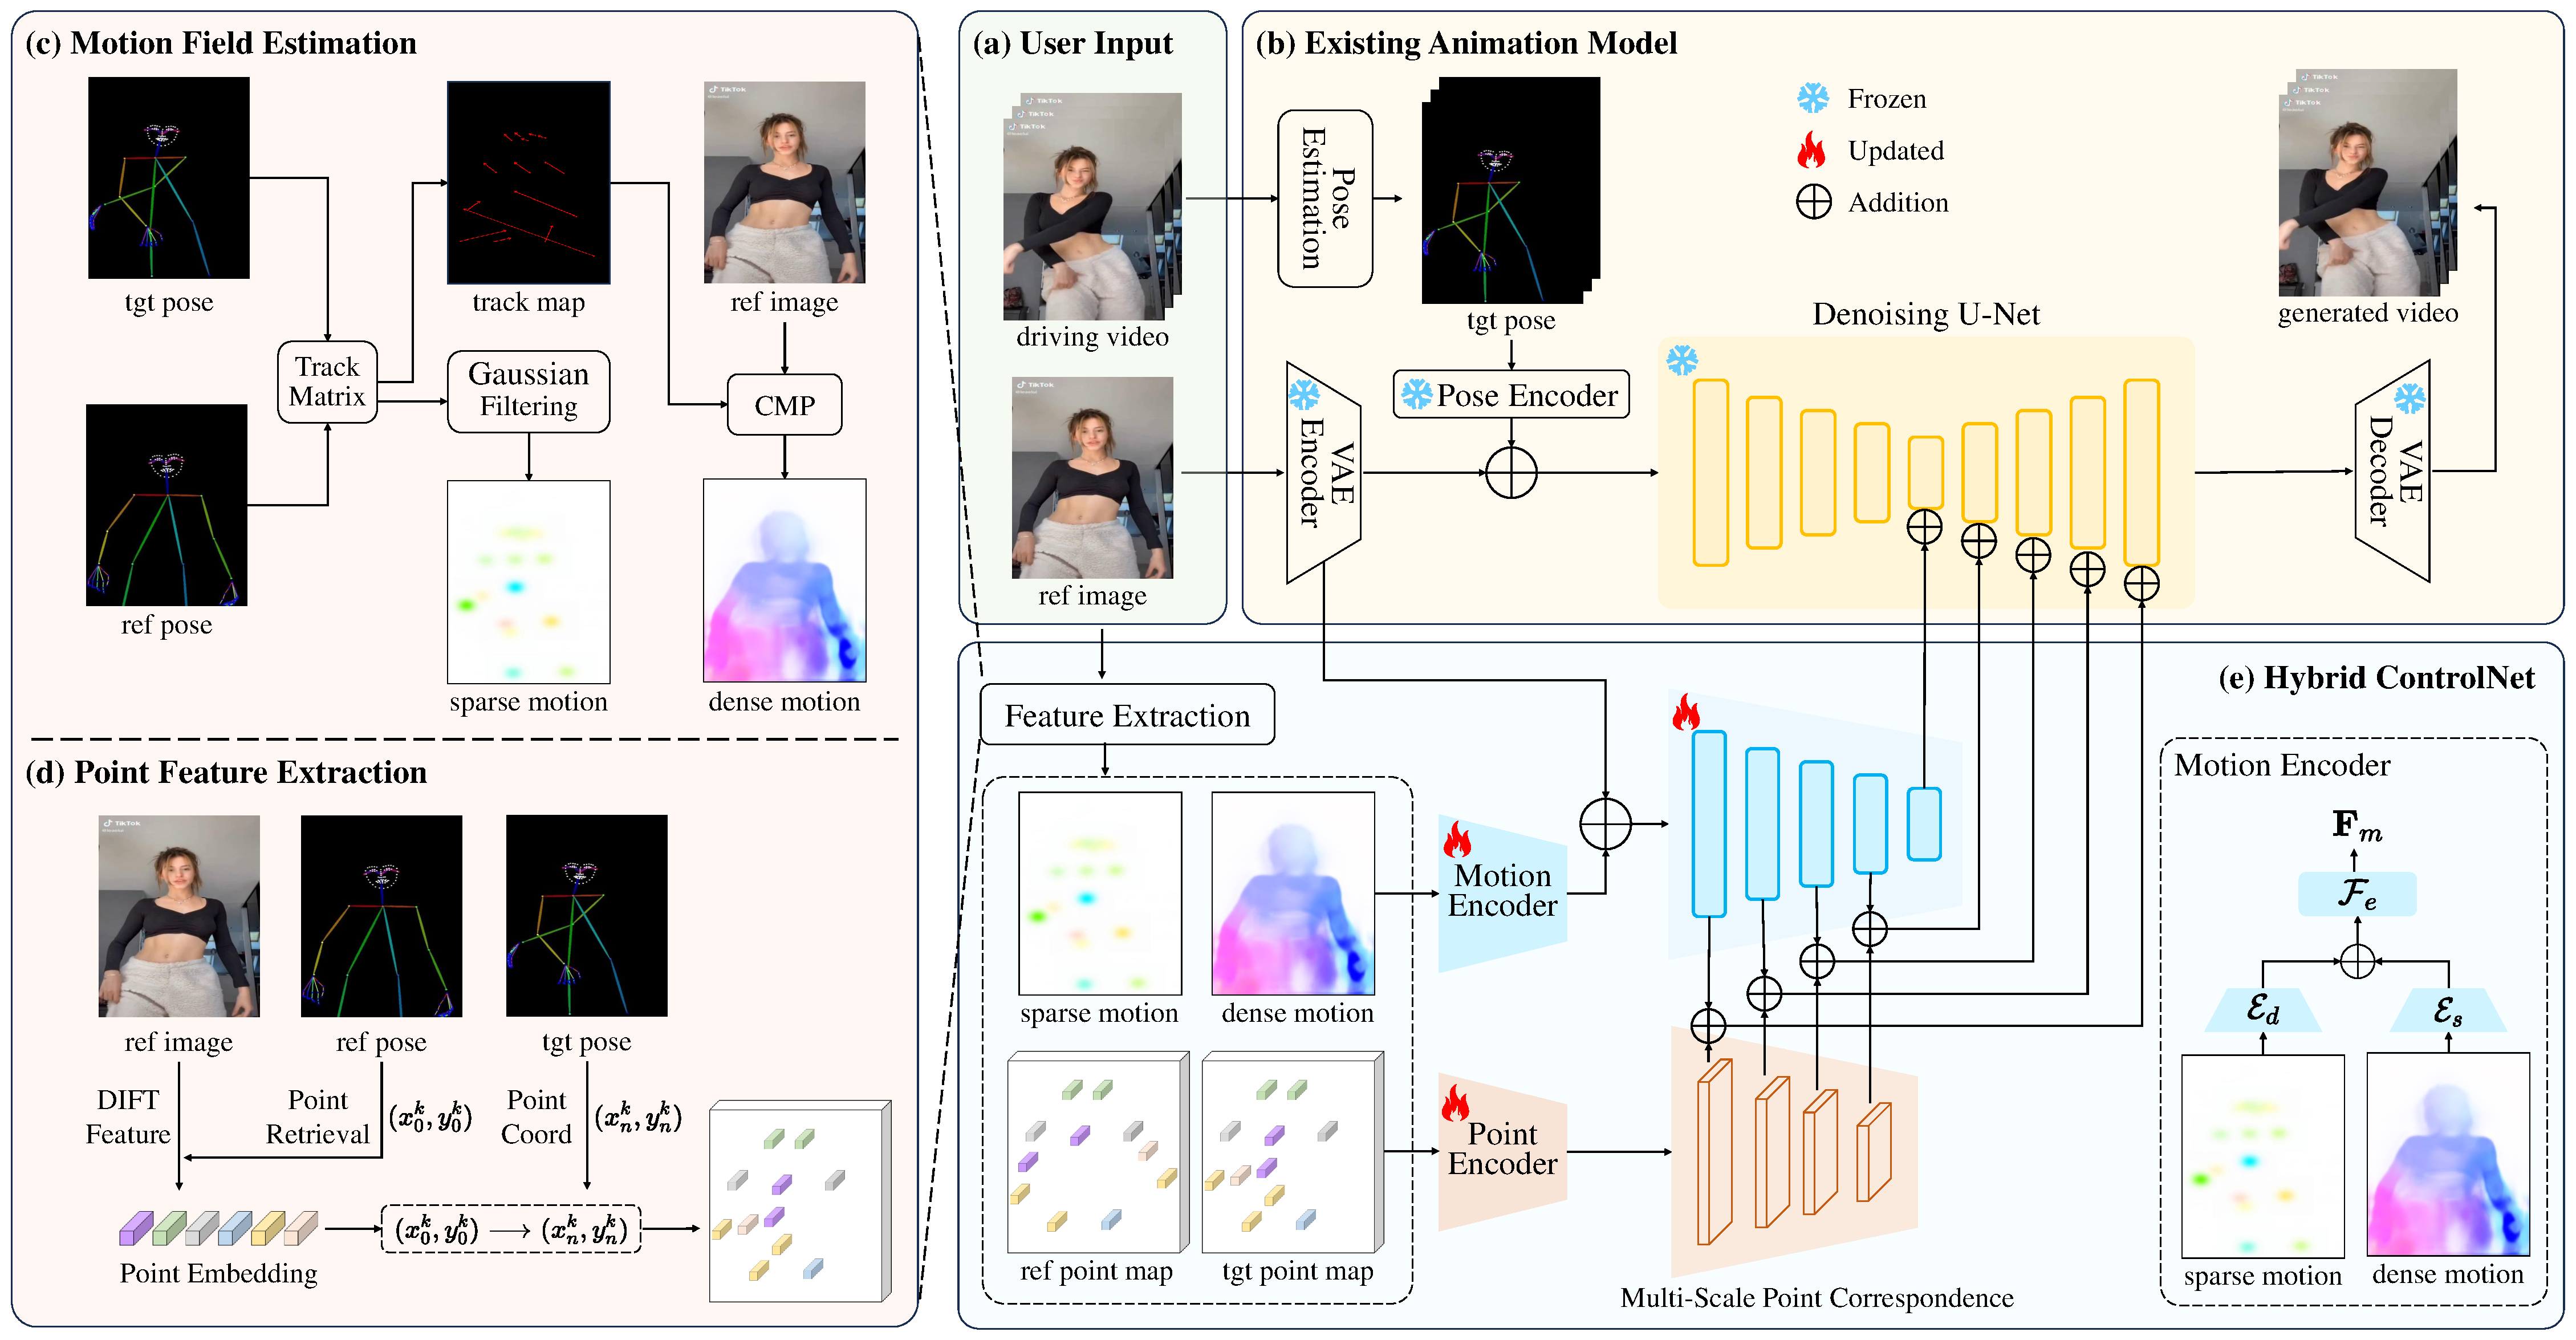
\includegraphics[width=1.0\columnwidth]{./image/pipeline.pdf}
    \vspace{-15pt}
    \caption{The overview of proposed DisPose.}
    \label{fig:pipeline}
\end{figure}
\section{DisPose}
Given a reference image $I_{\mathrm{ref}}\!\in\!\mathbb{R}^{3 \times H \times W}$ and a driving video $V\!\in\!\mathbb{R}^{N\times 3 \times H \times W}$. The core of our method is to disentangle efficient control guidance from only skeleton poses and reference images as shown in Figure~\ref{fig:pipeline}, which can be applied to existing human animation methods without additional dense inputs. We first introduce sparse and dense motion field guides in Sec.~\ref{sec: motion}. Then, we introduce reference-based keypoint correspondence in Sec.~\ref{sec: keypoint}. Finally, we introduce the pipeline of hybrid ControlNet in Sec~\ref{sec: controlnet}.
\subsection{Motion Field Guidance}
\label{sec: motion}

\textbf{Sparse Motion Field.}
We first estimate the skeleton pose by DWpose~\citep{yang2023dwpose} to obtain each frame's human key point coordinates. 
% Subsequently, the motion trajectory of all semantic points in the entire video is obtained and represented as
Subsequently, the key points of the reference image are used as starting points to track the motion displacement of all frames and represented as $P_{traj}\!=\!\{(x^k_n,y^k_n) \!\mid\! k=1\dots K, n=0\dots N\}$, where $P_{traj}$ denotes the trajectory map of the key point $k$ overall $N$ frames and $n = 0$ denotes the reference image. We calculate the track matrix $P_{s}$ as follows:
\begin{equation}
    \mathbf{P}_{s}=\{(x^k_n-x^k_{n-1}, y^k_n-y^k_{n-1}) \mid n=1\dots N\}\},
\end{equation}
% where $P_{t}$ denotes the trajectory map of the key point point $k$ over all $N$ frames, and the reference frame when $n = 0$.
where $K$ denotes the number of keypoints, $N$ denotes the number of frames, $\mathbf{P}_{s}$ denotes the trajectory map of keypoint k over all N frames, and $n = 0$ denotes the reference image.
To avoid training instability caused by overly sparse trajectory matrice, we then apply Gaussian filtering to enhance $\mathbf{P}_{s}$ to obtain the sparse motion field $\mathbf{F}_s\!\in\!\mathbb{R}^{(N-1)\times 2 \times H \times W}$ inspired by~\citep{yin2023dragnuwa, wang2024motionctrl}.

\textbf{Dense Motion Field.}
Considering that sparse control provides limited guidance and dense control is hard to obtain during inference,
% For the dense motion field, 
we transform dense guidance into the motion propagation from the reference frame to the target pose, instead of the dense signal of the target pose. Specifically, in the inference, we reconstruct the trajectory map $\mathbf{P}_{s}$ as the reference-based sparse optical flow $\mathbf{P}_{d}$ from the reference frame to each target pose as:
\begin{equation}
    \mathbf{P}_{d}=\{(x^k_n-x^k_{0}, y^k_n-y^k_{0}) \mid n=1\dots N\}\},
\end{equation}
We then predicted the reference-based dense motion filed $\mathbf{F}_d\!=\! \text{CMP}(P_{traj}, \mathbf{P}_{d}, I_{ref})\!\in\!\mathbb{R}^{(N-1)\times 2 \times H \times W}$ by condition motion propagation (CMP)~\citep{zhan2019self} based on the sparse optical flow $\mathbf{P}_{d}$ and the reference image $I_{ref}$.
CMP~\citep{zhan2019self} is a self-supervised learning-from-motion model that acquires an image and a sparse motion field and estimates the corresponding dense motion field.
Notably, the dense motion field $\mathbf{F}_d$ of each frame starts with the reference image, which avoids geometric constraints during inference.

To ensure motion estimation accuracy during training, we first extract the forward optical flow from the driving video using existing optical flow estimation models~\citep{teed2020raft, xu2023unifying}. We then use a watershed-based approach~\citep{zhan2019self} to sample the sparse optical flow $\mathbf{P}_{d}$ from the forward optical flow. See Appendix.~\ref{sec: appendix1} for details.

\textbf{Motion Encoder.} To leverage motion field as guidance, we introduce a motion encoder specifically designed for the optional flow, which includes sparse motion encoder $\mathcal{E}_s$, dense motion encoder $\mathcal{E}_d$ and feature fusion layer $\mathcal{F}_e$. $\mathcal{E}_d$ and $\mathcal{E}_s$ have the same structure and are multi-scale convolutional encoders with each stage built by \texttt{Conv-SiLU-ZeroConv}~\citep{zhang2023adding} as the basic block. The feature fusion layer $\mathcal{F}_e$ is a 2D convolution for fusing sparse motion features $\mathcal{E}_s(\mathbf{F}_s)$ and dense motion features $\mathcal{E}_d(\mathbf{F}_d)$. Finally, we compute the motion field guidance $\mathbf{F}_m$:
\begin{equation}
    \mathbf{F}_m = \mathcal{F}_e(\mathcal{E}_s(\mathbf{F}_s)+\mathcal{E}_d(\mathbf{F}_d))
\end{equation}

\subsection{Keypoint Correspondence}
\label{sec: keypoint}
\textbf{Point Feature Extraction.} 
To maintain a consistent appearance, it is crucial to correspond the content of the reference image with the motion trajectory. 
Specifically, we first extract the DIFT~\citep{tang2023emergent} features $\mathbf{D}$ of the reference image using the pre-trained image diffusion model. 

Subsequently, the keypoint embedding in the reference is obtained as $\mathbf{D}(x^k_0,y^k_0)$, where $(x^k_0,y^k_0)$ is retrieved from the reference pose.
% key point embeddings $\mathbf{D}(x^k_0,y^k_0)$ are retrieved from $\mathbf{D}$ by skeleton pose $(x^k_0, y^k_0)$.
Next, we initialize the keypoint correspondence map $\mathbf{F}_p$ with zero vectors and assign point embeddings according to the trajectory coordinates as:
\begin{equation}
\label{eq: v prob}
f^{ij}_n=\left\{\begin{array}{ll}
\mathbf{D}(x^k_0,y^k_0), & \mathrm{if} \quad i=x^k_n, j=y^k_n,  \\
0, & \mathrm{otherwise}.
\end{array}\right.
\end{equation}

Finally, we obtain the keypoint correspondence map $\mathbf{F}_p=\{f_n\!\mid\!n=1\dots N\} \!\in\!\mathbb{R}^{N\times D_p \times H \times W}$ for all frames, where $D_p$ is the feature dimension of the point embedding.

\textbf{Point Encoder.} 
To utilize the content correspondence of key points as guidance, we generate multi-scale correspondences of sparse point feature maps and make them compatible with the U-Net encoder of the {Hybrid ControlNet (Sec.4.3)}. 
% as detailed in F. 1.
We introduce the multi-scale point encoder $\mathcal{E}_p$ to maintain the key point content $\mathbf{F}_p$ from the reference image. The point encoder $\mathcal{E}_p$ consists of a series of learnable MLPs.
{
To seamlessly integrate into existing models, we extract intermediate features of the encoder of the hybrid Controlnet.
The multi-scale intermediate features of the Controlnet encoder are denoted as $\mathbf{E}^l_{enc}$, where $l$ denotes each U-Net block $l\!\in\![1, L]$.}
To match the spatial size of $\mathbf{E}^l_{enc}$, we apply downsampling to the feature map between the encoder layers. We compute the multi-scale keypoint correspondence as follows:
\begin{equation}
    \mathbf{F}_c^l = \mathcal{E}_p^l(\phi(\mathbf{F}_p, H^l, W^l)),
\end{equation}
where $(H^l, W^l)$ are denote the spatial dimension of the $l$-th U-Net block and $\phi$ means downsampling operation. Therefore, $\mathbf{F}_c^l$ shares the same size as $\mathbf{E}^l_{enc}$.
Finally, $\mathbf{F}_c$ are added elementwisely to the intermediate feature $\mathbf{E}^l_{enc}$ of the U-Net encoder as guidance: $\mathbf{E}^l_{enc}\!=\!\mathbf{E}^l_{enc}+\mathbf{F}_c^l$.


\subsection{Plug-and-play Hybrid ControlNet}
\label{sec: controlnet}
After obtaining motion field guidance and keypoint correspondence, we aim to integrate these control guidance seamlessly into the U-Net architecture of existing animation models.
Inspired by ControlNet~\citep{zhang2023adding}, We design a hybrid ControlNet $\mathcal{F}$ to provide additional control signals for the existing animation model as shown in Figure~\ref{fig:pipeline}(e).
% Specifically, we consider freeze denoising U-Net and pose encoder. 
Specifically, given an animation diffusion model based on the U-Net architecture, we freeze all its modules while allowing the motion encoder, point encoder and hybrid ControlNet to be updated during training. 
Subsequently, $\mathbf{F}_m$ is added to the noise latent before being input into the hybrid ControlNet. Considering the high sparsity of the point feature $\mathbf{F}_c$, we correspondingly add $\mathbf{F}_c$ to the input of the convolutional layer. Notably, the U-Net encoder intermediate feature $\mathbf{E}_{enc}$ in Sec.~\ref{sec: keypoint} is from hybrid ControlNet rather than denoising U-Net. Finally, 
the control condition is computed as:
\begin{equation}
    \boldsymbol{r}=\mathcal{F}(\boldsymbol{z}_{{t}} \mid \mathbf{F}_m, \mathbf{F}_c, {t})
\end{equation}
where $\boldsymbol{r}$ is a set of condition residuals added to the residuals for the middle and upsampling blocks in the denoising U-Net.
\section{Experiments}
\label{sec:experiments}

We validate our approach empirically, showing that our Monarch matrix parametrization achieves a favorable efficiency--accuracy tradeoff compared to baselines on a wide range of domains (text, images, PDEs, MRI), in three settings (E2E training, S2D training, and D2S fine-tuning):
\begin{itemize}[leftmargin=*,nosep,nolistsep,noitemsep]
\item
In \cref{subsec:benchmark_tasks}, on image classification and language modeling benchmarks, such as ViT / MLP Mixer on ImageNet and GPT-2 on Wikitext-103, Monarch is 2$\times$ faster to train than dense models, while achieving the same accuracy / perplexity. In \cref{subsec:pde_mri}, in scientific and medical domains where special transforms (Fourier) are common, Monarch outperforms Fourier transform based methods on PDE solving, with up to 40\% lower error, and on MRI reconstruction attains up to 15\% higher pSNR and 3.8\% higher SSIM.
\item In \cref{subsec:pde_mri}, we show that on the large OpenWebText dataset, reverse sparsification (training with Monarch weight matrices for most of the time, then transitioning to dense weight matrices) speeds up the pretraining of GPT-2 models by 2$\times$ compared to the dense model, with no loss in upstream or downstream quality.
Moreover, reverse sparsification speeds up BERT pretraining by 23\% even compared to the implementation from Nvidia that set the MLPerf~\citep{mattson2020mlperf} 1.1 record.
\item In \cref{subsec:finetuning}, as a proof of concept, we demonstrate that our Monarch approximation algorithm can improve fine-tuning efficiency for pretrained models. We show that compressing BERT to a Monarch matrix model performs comparably to a finetuned dense model on GLUE, with 2$\times$ fewer parameters and 1.7$\times$ faster finetuning speed.
\end{itemize}

\subsection{End-to-End Training}
\label{subsec:e2e_training}
\subsubsection{Benchmark Tasks: Image Classification, Language Modeling}
\label{subsec:benchmark_tasks}

We show that replacing dense matrices with Monarch matrices in ViT, MLP-Mixer, and
GPT-2 can speed up training by up to 2$\times$ without sacrificing model quality in~\cref{table:pretrain,table:gpt_pretrain}.

\textbf{Setup.} We use the popular vision benchmark, ImageNet~\citep{deng2009imagenet}. We choose recent popular Vision Transformer~\citep{dosovitskiy2020image}, and MLP-Mixer~\citep{tolstikhin2021mlp} as representative base dense models.
For language modeling, we evaluate GPT-2~\citep{radford2019language} on WikiText-103~\citep{merity2016pointer}.

\begin{table}[h]
  \small
  \centering
  \vspace{-2mm}
  \caption{\label{table:pretrain}The performance of Monarch matrices and ViT / MLP-Mixer on ImageNet, including the number of parameters and FLOPs. We measure the Top-1 accuracy and the training time speedup compared to the corresponding dense model. %
  \vspace{2mm}
  }
  \iftoggle{arxiv}{}{
  \resizebox{\linewidth}{!}
  }
  {
  \setlength{\tabcolsep}{3pt}
  \vspace{3em}
  \begin{tabular}{@{}c||ccccccc@{}}
  \specialrule{.15em}{.05em}{.05em}
    Model&\multicolumn{1}{c}{ImageNet acc.}&\multicolumn{1}{c}{Speedup} &\multicolumn{1}{c}{Params} & \multicolumn{1}{c}{FLOPs} \\
    \specialrule{.15em}{.05em}{.05em}
    Mixer-S/16& 74.0& - & 18.5M & 3.8G \\
    Monarch-Mixer-S/16& 73.7& 1.7$\times$ & 7.0M & 1.5G \\
    Mixer-B/16& 77.7& - & 59.9M & 12.6G \\
    Monarch-Mixer-B/16& 77.8& 1.9$\times$ & 20.9M & 5.0G \\
    \specialrule{.15em}{.05em}{.05em}
    ViT-S/16& 79.4 & - & 48.8M & 9.9G \\
    Monarch-ViT-S/16& 79.1 & 1.9$\times$ & 19.6M & 3.9G \\
    ViT-B/16& 78.5 & - & 86.6M  & 17.6G \\
    Monarch-ViT-B/16& 78.9 & 2.0$\times$ & 33.0M & 5.9G \\
    \specialrule{.15em}{.05em}{.05em}
  \end{tabular}
  }
\end{table}

\begin{table}[h]
  \small
  \centering
  \vspace{-3mm}
  \caption{\label{table:gpt_pretrain} Performance of Monarch matrices and GPT-2-Small/Medium on WikiText-103, including the \# of parameters and FLOPs. Monarch achieves similar perplexity (ppl) but 2.0$\times$ faster.}
  \vspace{1mm}
  \iftoggle{arxiv}{}{
    \resizebox{0.95\linewidth}{!}
  }
  {
\setlength{\tabcolsep}{5pt}
\begin{tabular}{c||cccc}
\specialrule{.15em}{.05em}{.05em}
\multirow{1}{*}{{ Model} } & \multicolumn{1}{c}{\multirow{1}{*}{PPL}}
                              & \multicolumn{1}{c}{\multirow{1}{*}{Speedup}}
                              & \multicolumn{1}{c}{\multirow{1}{*}{Params}}
                              & \multicolumn{1}{c}{\multirow{1}{*}{FLOPs}}\\
\specialrule{.15em}{.05em}{.05em}
GPT-2-Small &  20.6 & - & 124M& 106G\\
Monarch-GPT-2-Small& 20.7  & 1.8$\times$ &72M & 51G\\
\specialrule{.15em}{.05em}{.05em}
GPT-2-Medium &  20.9 & - & 355M& 361G\\
Monarch-GPT-2-Medium& 20.3  & 2.0$\times$ &165M & 166G\\
\specialrule{.15em}{.05em}{.05em}
\end{tabular}
}
\vspace{-2mm}
\end{table}


\subsubsection{PDE solving and multi-coil MRI reconstruction}
\label{subsec:pde_mri}

Many scientific or medical imaging tasks rely on specialized transforms such as the
Fourier transform.
We show that replacing the fixed Fourier transform with the more expressive
Monarch matrices yields higher model quality (lower reconstruction error) with
comparable model speed.

\textbf{Solving PDEs with Monarch Neural Operators.}
We follow the experimental setting in FNO~\citep{li2020fourier} and apply a Monarch--based neural operator to the task of solving the Navier--Stokes PDE. Compared to baseline U-Nets~\citep{ronneberger2015u}, TF-Nets~\citep{wang2020towards}, ResNets~\citep{he2016deep} and FNOs~\cite{li2020fourier}, neural operators based on Monarch improve solution accuracy across spatial resolutions by up to $40\%$ (Table \ref{table:pde}).  





\paragraph{Non-periodic boundary conditions.} Traditional spectral methods based on Fourier transform work best with periodic boundary conditions and forcing terms. However, PDEs of practical interest often exhibit non--periodic or even unknown boundary conditions. Monarch operators are not constrained to the Fourier transform and can thus still learn the solution operator with excellent accuracy.

\begin{table}[h!] 
\scriptsize
\vspace{-4mm}
\caption{\label{table:pde}Benchmarks on Navier-Stokes (fixing resolution 64 × 64 for both training and testing).
Decreasing the viscosity coefficient $\nu$ makes the dynamics more chaotic.
}
\vspace{1mm}
\centering
\iftoggle{arxiv}{}{
  \resizebox{0.9\linewidth}{!}
}
{
\renewcommand{\arraystretch}{1}
\begin{tabular}{ c||ccc }
\specialrule{.15em}{.05em}{.05em}
Model & $v = 10^{-3}$  &  $v = 10^{-4}$ & $v = 10^{-5}$\\
\specialrule{.15em}{.05em}{.05em}
U-Net & 0.025  & 0.205  &   0.198\\
TF-Net  & 0.023  & 0.225 &  0.227 \\
ResNet & 0.070 &  0.287 &  0.275 \\
FNO & 0.017  & 0.178 & 0.155\\
Monarch-NO & \textbf{0.010} & \textbf{0.145} & \textbf{0.136} \\
\specialrule{.15em}{.05em}{.05em}
\end{tabular}
}
\textbf{\vspace{-3mm}}
\end{table}

\textbf{Accelerated MRI Reconstruction.} We characterize the utility of Monarch-based FFT operations for accelerated MRI reconstruction, a task which requires methods with both structured Fourier operators and dealiasing properties to recover high quality images. On the clinically-acquired 3D MRI SKM-TEA dataset \citep{desai2021skm}, Monarch-SENSE (mSENSE) enhances image quality by over 1.5dB pSNR and 2.5\% SSIM compared to zero-filled SENSE and up to 4.4dB and 3.8\% SSIM compared to U-Net baselines in data-limited settings. Setup details are available in~\cref{sec:experiment_details_mri}.

\paragraph{Expressive FFT.} By definition, standard IFFT in zero-filled SENSE cannot dealias the signal, resulting in artifacts in the reconstructed image. mSENSE replaces the inverse FFT (IFFT) operation in standard SENSE with learnable Monarch matrices. Thus, mSENSE preserves the structure of the Fourier transform while learning to reweight frequencies to suppress aliasing artifacts. Across multiple accelerations, mSENSE achieved up to +1.5dB and 2.5\% improvement in peak signal-to-noise ratio (pSNR) and structural similarity (SSIM), respectively (Table~\ref{table:mri}).

\paragraph{Data Efficiency.} While CNNs have shown promise for MRI reconstruction tasks, training these networks requires extensive amounts of labeled data to avoid overfitting. However, large data corpora are difficult to acquire in practice. mSENSE can be trained efficiently with limited supervised examples. In few shot settings, mSENSE can outperform U-Net by +4.4dB ($\approx$15\%) and 3.8\% SSIM (Table~\ref{table:mri-data-limited}). 







\begin{table}[h!] 
\scriptsize
\vspace{-3mm}
\caption{\label{table:mri}Mean $\pm$ standard error of the mean of conventional and Monarch-SENSE (mSENSE) on dual-echo (E1,E2) MRI reconstruction at multiple acceleration factors (Acc.).
}
\vspace{1mm}
\centering
\iftoggle{arxiv}{}{
  \resizebox{\linewidth}{!}
}
{
\renewcommand{\arraystretch}{1.2}
\begin{tabular}{c||ccccc}
\specialrule{.15em}{.05em}{.05em}
  & & \multicolumn{2}{c}{pSNR (dB) ($\uparrow$)} & \multicolumn{2}{c}{SSIM ($\uparrow$)} \\
  Acc. & Model &             E1 &             E2 &                E1 &                E2 \\
\specialrule{.15em}{.05em}{.05em}
\multirow{2}{*}{2} & SENSE &  32.8$\pm$0.2 &  35.4$\pm$0.2 &  0.871$\pm$0.003 &  0.865$\pm$0.003 \\
  & mSENSE &  \textbf{34.3$\pm$0.2} &  \textbf{36.6$\pm$0.2} &  \textbf{0.886$\pm$0.002} &  \textbf{0.882$\pm$0.003} \\
\specialrule{.15em}{.05em}{.05em}
\multirow{2}{*}{3} & SENSE &  30.9$\pm$0.2 &  33.5$\pm$0.2 &  0.819$\pm$0.004 &  0.795$\pm$0.004 \\
  & mSENSE &  \textbf{32.3$\pm$0.2} &  \textbf{34.6$\pm$0.2} &  \textbf{0.843$\pm$0.003} &  \textbf{0.820$\pm$0.004} \\
\specialrule{.15em}{.05em}{.05em}
\multirow{2}{*}{4} & SENSE &  30.1$\pm$0.2 &  32.8$\pm$0.2 &  0.789$\pm$0.004 &  0.753$\pm$0.005 \\
  & mSENSE &  \textbf{31.2$\pm$0.2} &  \textbf{33.5$\pm$0.2} &  \textbf{0.812$\pm$0.003} &  \textbf{0.767$\pm$0.005} \\
\specialrule{.15em}{.05em}{.05em}
\end{tabular}
}
\end{table}

\begin{table}[h!] 
\scriptsize
\vspace{-5mm}
\caption{\label{table:mri-data-limited}Impact of number of training examples ($N$) on dual-echo MRI reconstruction at 2x acceleration.
}
\vspace{1mm}
\centering
\iftoggle{arxiv}{}{
  \resizebox{\linewidth}{!}
}
{
\renewcommand{\arraystretch}{1.2}
\begin{tabular}{c||ccccc}
\specialrule{.15em}{.05em}{.05em}
  &  & \multicolumn{2}{c}{pSNR (dB) ($\uparrow$)} & \multicolumn{2}{c}{SSIM ($\uparrow$)} \\
  $N$ & Model &            E1 &            E2 &               E1 &               E2 \\
\specialrule{.15em}{.05em}{.05em}
N/A & SENSE &  32.8$\pm$0.2 &  35.4$\pm$0.2 &  0.871$\pm$0.003 &  0.865$\pm$0.003 \\
\specialrule{.15em}{.05em}{.05em}
\multirow{2}{*}{1} & U-Net &  29.4$\pm$0.2 &  34.4$\pm$0.3 &  0.848$\pm$0.004 &  0.857$\pm$0.004 \\
  & mSENSE &  \textbf{33.8$\pm$0.2} &  \textbf{36.0$\pm$0.2} &  \textbf{0.886$\pm$0.003} &  \textbf{0.867$\pm$0.003} \\
\specialrule{.15em}{.05em}{.05em}
\multirow{2}{*}{2} & U-Net &  29.9$\pm$0.3 &  35.1$\pm$0.3 &  0.858$\pm$0.003 &  0.871$\pm$0.003 \\
  & mSENSE &  \textbf{34.0$\pm$0.2} &  \textbf{36.4$\pm$0.2} &  \textbf{0.883$\pm$0.002} &  \textbf{0.877$\pm$0.003} \\
\specialrule{.15em}{.05em}{.05em}
\multirow{2}{*}{3} & U-Net &  31.0$\pm$0.3 &  35.2$\pm$0.3 &  0.866$\pm$0.003 &  0.867$\pm$0.004 \\
  & mSENSE &  \textbf{33.9$\pm$0.2} & \textbf{ 36.5$\pm$0.2} &  \textbf{0.882$\pm$0.002} & \textbf{0.878$\pm$0.003} \\
\specialrule{.15em}{.05em}{.05em}
\multirow{2}{*}{5} & U-Net &  31.4$\pm$0.3 &  35.6$\pm$0.2 &  0.877$\pm$0.002 &  0.870$\pm$0.003 \\
  & mSENSE &  \textbf{33.9$\pm$0.2} &  \textbf{36.5$\pm$0.2} &  \textbf{0.881$\pm$0.002} &  \textbf{0.877$\pm$0.003} \\
\specialrule{.15em}{.05em}{.05em}
\end{tabular}
}
\end{table}




\subsection{Sparse-to-Dense Training (reverse sparsification)}
\label{subsec:s2d_training}
\paragraph{GPT-2 pretraining.}
On the large OpenWebtext dataset~\citep{Gokaslan2019OpenWeb}, we train a GPT-2 model with Monarch weight
matrices for 90\% of the training iterations, then relax the constraint on the
weight matrices and train them as dense matrices for the remaining 10\% of the
iterations.
We call this technique ``reverse sparsification.''
Previous sparse training techniques often don't speed up training, whereas our
hardware-efficient Monarch matrices do.
Therefore we can use them as an intermediate step to pretrain a large language
model (GPT-2) in 2$\times$ less time. We also evaluate its downstream quality on zero-shot generation from~\citep{eval-harness} and classification tasks from~\citep{zhao2021calibrate}, achieving comparable performance to the dense counterparts (\cref{table:gpt_finetune}). 

\begin{table}[h]
  \small
  \centering
  \vspace{-3mm}
  \caption{\label{table:gpt_finetune}The performance (accuracy) of GPT-2-medium trained with Monarch reverse sparsification and with conventional dense training on text classification benchmarks.}
  \setlength{\tabcolsep}{5pt}
  \vspace{1em}
  \iftoggle{arxiv}{}{
    \resizebox{\linewidth}{!}
  }
  {
  \begin{tabular}{@{}c||ccc@{}}
    \specialrule{.15em}{.05em}{.05em}
    Model&\multicolumn{1}{c}{OpenWebText (ppl)}&\multicolumn{1}{c}{Speedup}& \multicolumn{1}{c}{Classification (avg acc)} \\
    \specialrule{.15em}{.05em}{.05em}
    GPT-2m& 18.0 & - & 38.9 \\
    Monarch-GPT-2m& 18.0 & 2$\times$ & 38.8 \\
    \specialrule{.15em}{.05em}{.05em}
  \end{tabular}
  }
  \vspace{-3mm}
\end{table}


In \cref{fig:reverse_sparsification_bar}, we show the training time of the dense GPT-2 model, along with
the Monarch GPT-2 model.
After training the Monarch model for 90\% of the time, in the
last 10\% of the training steps, by transitioning to dense weight matrices, the model is able to reach the same 
performance of another model that was trained with dense weight matrices from
scratch.
By training with Monarch matrices for 90\% of the time, we reduce the total training time by 2$\times$.

\paragraph{BERT pretraining.}
On the Wikipedia + BookCorpus datasets~\citep{zhu2015aligning}, we train a BERT-large model with Monarch weight matrices for 70\% of the time and transition to dense weight matrices for the remaining 30\% of the time, which yields the same pretraining loss as conventional dense training.
In \cref{table:bert_speed}, we compare the total training time to several baseline implementations: the widely-used implementation from HuggingFace~\citep{wolf-etal-2020-transformers}, the more optimized implementation from Megatron~\citep{shoeybi2019megatron}, and the most optimized implementation we know of from Nvidia that was used to set MLPerf 1.1 training speed record. Our method is 3.5x faster than HuggingFace and 23\% faster than Nvidia's MLPerf 1.1 implementation\footnote{Our result is not an official MLPerf submission. We train BERT for both phase 1 (sequence length 128) and phase 2 (sequence length 512) according to the standard BERT training recipe\cite{devlin2018bert}, while MLPerf only measures training time for phase 2.}.
Experiment details are in~\cref{subsec:bert_details}.

\begin{table}[h]
  \small
  \centering
  \caption{\label{table:bert_speed}The total training time of BERT-large trained with Monarch reverse sparsification and with conventional dense training on 8 A100-40GB GPUs (DGX A100). Training consists of two phases, phase 1 with sequence length 128 and phase 2 with sequence length 512. Monarch training is 3.5x faster than HuggingFace and 23\% faster than Nvidia's MLPerf 1.1 implementation.}
  \vspace{1em}
  \iftoggle{arxiv}{}{
    \resizebox{\linewidth}{!}
  }
  {
    \begin{tabular}{@{}c||c@{}}
      Implementation & Training time (h)  \\ \hline
      HuggingFace &  84.5 \\
      MegaTron & 52.5 \\
      Nvidia MLPerf 1.1 & 30.2 \\
      Nvidia MLPerf 1.1 + DeepSpeed & 29.3 \\
      Monarch (ours) & \textbf{23.8} \\
    \end{tabular}
  }
  \vspace{-3mm}
\end{table}

\subsection{Dense-to-Sparse Fine-tuning}
\label{subsec:finetuning}

\begin{figure}[t]
  \centering
  \vspace{-3mm}
  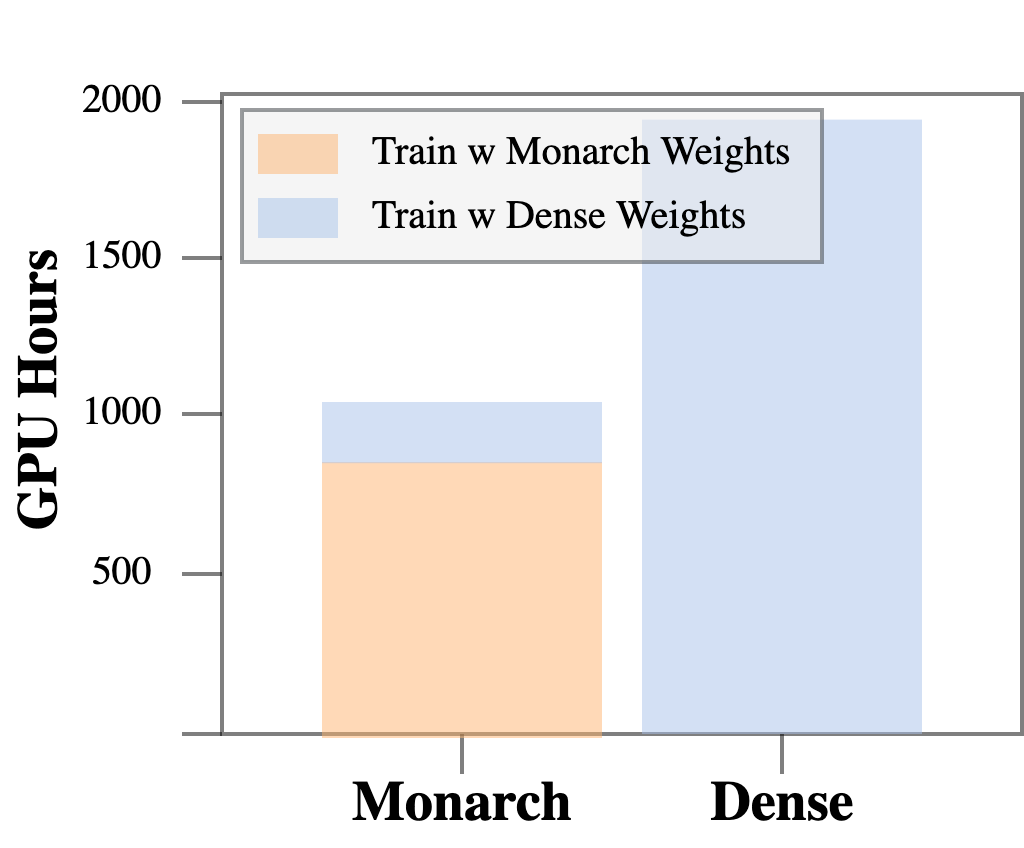
\includegraphics[width=.3\textwidth]{figures/rv_bar_temp.png}
  \vspace{-3mm}
  \caption{\label{fig:reverse_sparsification_bar}Time required (in A100 GPU hours) to reach the same perplexity (18.0)
    for GPT-2-small on OpenWebText.
    With ``reverse sparsification'', Monarch can speed up
    GPT-2 training by 2$\times$.\vspace{-1em}}
\end{figure}

We show that our Monarch approximation algorithm allows us to efficiently use
pretrained models, such as speeding up BERT finetuning on GLUE.

\paragraph{BERT finetuning.}
We take the BERT pretrained weights, approximate them with Monarch matrices,
and finetune the resulting model on the 9 GLUE tasks.
The results in \cref{table:bert_glue} shows that we obtain a Monarch finetuned
model with similar quality to the dense BERT model, but with 1.7$\times$ faster
finetuning speed.
This serves as a proof of concept, and we expect further speedup if additional model compression techniques are applied (e.g., quantization, kernel fusion).




\begin{table}[h]
  \small
  \centering
  \vspace{-5mm}
  \caption{\label{table:bert_glue}The performance of Monarch matrices in
    finetuning BERT on GLUE.}
  \setlength{\tabcolsep}{5pt}
  \vspace{1em}
  \iftoggle{arxiv}{}{
    \resizebox{\linewidth}{!}
  }
  {
  \begin{tabular}{@{}c||ccccccc@{}}
  \specialrule{.15em}{.05em}{.05em}
    Model&\multicolumn{1}{c}{GLUE (avg)}&\multicolumn{1}{c}{Speedup} &\multicolumn{1}{c}{Params} & \multicolumn{1}{c}{FLOPs} \\
    \specialrule{.15em}{.05em}{.05em}
    BERT-base & 78.6& - & 109M & 11.2G \\
    Monarch-BERT-base& 78.3& 1.5$\times$ & 55M & 6.2G  \\
    BERT-large & 80.4 & - & 335M & 39.5G \\
    Monarch-BERT-large & 79.6 & 1.7$\times$ & 144M & 14.6G  \\
    \specialrule{.15em}{.05em}{.05em}
  \end{tabular}
  }
  \vspace{-3mm}
\end{table}




\vspace{-7pt}
\section{Conclusion}
\vspace{-8pt}
In this work, we study Continual Self-Supervised Learning (CSSL), the problem of learning a set of tasks without labels continually. We make two important contributions for the SSL and CL communities: (i) we present \name{}, a simple and effective framework for CSSL that shows how SSL methods and losses can be seamlessly reused to learn continually, and (ii) we perform a comprehensive analysis of CSSL, leading to the emergence of  interesting properties of SSL methods.

\noindent\textbf{Limitations.} Although \name{} shows exciting performance, it has some limitations. First, it is applicable in settings where task boundaries are provided. Second, our framework increases the amount of computational resources needed for training by roughly 30\%, both in terms of memory and time. Finally, \name{} does not perform clustering, meaning that it is unable to directly learn a mapping from data to latent classes, and thus needs either a linear classifier trained with supervision, or some clustering algorithm.

\noindent\textbf{Broader impact.} The capabilities of supervised CL agents are bounded by the need for human-produced annotations. CSSL models can potentially improve without the need for human supervision. This facilitates the creation of powerful AIs that may be used for malicious purposes such as discrimination and surveillance. Also, since in CSSL the data is supposed to come from a non-curated stream, the model may be affected by biases in the data. This is problematic because biases are then be transferred to downstream tasks.

\small{\noindent\textbf{Acknowledgements.} This work was supported by the European Institute of Innovation \& Technology (EIT) and the H2020 EU project SPRING, funded by the European Commission under GA 871245. It was carried out under the ``Vision and Learning joint Laboratory" between FBK and UNITN. Karteek Alahari was funded by the ANR grant AVENUE (ANR-18-CE23-0011). Julien Mairal was funded by the ERC grant number 714381 (SOLARIS project) and by ANR 3IA MIAI@Grenoble Alpes (ANR-19-P3IA-0003). Xavier Alameda-Pineda was funded by the ARN grant ML3RI (ANR-19-CE33-0008-01). This project was granted access to the HPC resources of IDRIS under the allocation 2021-[AD011013084] made by GENCI.}






% change the section to A, B, C
\renewcommand\thesection{\Alph{section}}
\renewcommand\thefigure{\Alph{figure}}
\renewcommand\thetable{\Alph{table}}
\setcounter{section}{0}
\setcounter{figure}{0}
\setcounter{table}{0}

\section*{Appendix}

\section{PyTorch-like pseudo-code}
We provide a PyTorch-like pseudo-code of our method. As you can see, \name{} is simple to implement and does not add much complexity to the base SSL method. In this snippet, the losses are made symmetric by summing the two contributions. In some cases, the two losses are averaged instead. In \name{}, we symmetrize in the same way as the base SSL method we are considering.
\begin{algorithm}[h]

   \caption{PyTorch-like pseudo-code for \name{}.}
   \label{algo:DINO}
    \definecolor{codeblue}{rgb}{0.25,0.5,0.5}
    \definecolor{codekw}{rgb}{0.85, 0.18, 0.50}
    \lstset{
      basicstyle=\fontsize{7.2pt}{7.2pt}\ttfamily,
      commentstyle=\fontsize{7.2pt}{7.2pt}\color{codeblue},
      keywordstyle=\fontsize{7.2pt}{7.2pt}\color{codekw},
    }
\begin{lstlisting}[language=python]
# aug: stochastic image augmentation
# f: backbone and projector
# frozen_f: frozen backbone and projector
# g: CaSSLe's predictor
# loss_fn: any SSL loss in Tab. 1 (main paper)

# PyTorchLightning handles loading and optimization
def training_step(x):

    # correlated views
    x1, x2 = aug(x), aug(x)

    # forward backbone and projector
    z1, z2 = f(x1), f(x2)

    # optionally forward predictor...

    # compute SSL loss (symmetric)
    ssl_loss = loss_fn(z1, z2) \\
             + loss_fn(z2, z1)

    # forward frozen backbone and projector
    z1_bar, z2_bar = frozen_f(x1), frozen_f(x2)

    # compute distillation loss (symmetric)
    distill_loss = loss_fn(g(z1), z1_bar) \\
                 + loss_fn(g(z2), z2_bar)
    
    # no hyperparameter for loss weighting
    return ssl_loss + distill_loss
\end{lstlisting}
\end{algorithm}

\section{Derivation of distillation losses}
In this section, we derive distillation losses from the SSL losses in Tab. 1 of the main paper, starting from the definition of our distillation loss:
\begin{equation}
    \mathcal{L}_D(\zvect, \bar{\zvect}) = \mathcal{L}_{SSL} (g(\zvect), \bar{\zvect}),
\end{equation}
where $z$ and $\bar{z}$ are the representations of the current and frozen encoder, and $g$ is \name{}'s predictor network implemented as a two layer MLP with 2048 hidden neurons and ReLU activation.
\paragraph{Contrastive based.} Our distillation loss based on contrastive learning is implemented as follows:
\begin{equation}
    \mathcal{L}(z_i, \bar{z}_i) = -\log \frac{\exp \left(\operatorname{sim}\left(\zvect_i, \bar{\zvect}_i\right) / \tau\right)}{\sum_{\zvect_j \in \bar{\eta}(i)} \exp \left(\operatorname{sim}\left(\zvect_i, \zvect_{j}\right) / \tau\right)},
\end{equation}
where $\bar{\eta}(i)$ is the set of negatives for the sample with index $i$ in the batch. Note that the negatives are drawn both from the predicted and frozen features.
\paragraph{MSE based.} This distillation loss is simply the MSE between the predicted features and the frozen features:
\begin{equation}
    \mathcal{L}(z, \bar{z}) = -||g(\zvect) -  \bar{\zvect}||^2_2 .
\end{equation}
It can be implemented with the cosine similarity as stated in the main manuscript.
\paragraph{Cross-entropy based.} The cross-entropy loss, when used for distillation in an unsupervised setting, makes sure that the current encoder is able to assign samples to the frozen centroids (or prototypes) consistently with the frozen encoder:
\begin{equation}
    \mathcal{L}(z, \bar{z}) = -\sum_{d} \bar{\avect}_{d} \log \frac{\exp \left(\operatorname{sim}\left( g(\zvect), \cvect^{t-1}_{d}\right) / \tau\right)}{\sum_k \exp \left(\operatorname{sim}\left(g(\zvect), \cvect^{t-1}_k\right) / \tau\right)} 
\end{equation}
where:
\begin{equation}
    \bar{\avect}= \frac{\exp \left(\operatorname{sim}\left( \bar{\zvect}, \cvect^{t-1}_{d}\right) / \tau\right)}{\sum_k \exp \left(\operatorname{sim}\left(\bar{\zvect}, \cvect^{t-1}_k\right) / \tau\right)},
\end{equation}
and the set of frozen prototypes is denoted as follows: $\mathbf{C}^{t-1} = \left\{\mathbf{c}^{t-1}_{1}, \ldots, \mathbf{c}^{t-1}_{K}\right\}$.
 
\paragraph{Cross-correlation based.} We consider Barlow Twins'~ \cite{zbontar2021barlow} implementation of this objective. For VICReg~\cite{bardes2021vicreg} we only consider the invariance term. As a distillation loss, the cross-correlation matrix is computed with the predicted and frozen features:

\begin{equation}
    \mathcal{L}(z, \bar{z}) = \sum_{u}\left(1-\bar{\mathcal{C}}_{u v}\right)^{2}+\lambda \sum_{u} \sum_{v \neq u} \bar{\mathcal{C}}_{u v}^{2} ,
\end{equation}
where:
\begin{equation}
    \bar{\mathcal{C}}_{u v} = \frac{\sum_{i} g(\zvect_{i, u}) \bar{\zvect}_{i, v}}{\sqrt{\sum_{i}g\left(\zvect_{i, u}\right)^{2}}. \sqrt{\sum_{i}\left(\bar{\zvect}_{i, v}\right)^{2}}}.
\end{equation} 

\section{Further discussion and implementation details of the baselines}
\paragraph{Selection.} When evaluating our framework, we try to compare with as many existing related methods as possible. However, given that SSL models are computationally intensive, it was not possible to run all baselines and methods in all the CL settings we considered. As mentioned in the main manuscript, we choose eight baselines (seven related methods + fine-tuning) belonging to three CL macro-categories, and test them on CIFAR100 (class-incremental) in combination with three SSL methods. The selection was based on the ease of adaptation to CSSL and the similarity to our framework.

\begin{table*}[ht]
\centering
\scriptsize
\captionsetup{type=table}
\captionsetup{width=.99\linewidth}
\caption{Linear evaluation top-1 accuracy on DomainNet (6 tasks, domain-incremental setting) w/ and w/o \name{}. The sequence of tasks is Real$\rightarrow$Quickdraw$\rightarrow$Painting$\rightarrow$Sketch$\rightarrow$Infograph$\rightarrow$Clipart. ``Aw.'' stands for task-aware, ``Ag,'' for task-agnostic.}
\label{tab:domain-incremental-task-agnostic}
\vspace{-2px}
\begin{tabular}{lccccccccccccccc}
\toprule
\multirow{2}[1]{*}{\textbf{Method}} & \multirow{2}[1]{*}{\textbf{Strategy}} & \multicolumn{2}{c}{\textbf{Real}} & \multicolumn{2}{c}{\textbf{Quickdraw}} & \multicolumn{2}{c}{\textbf{Painting}} & \multicolumn{2}{c}{\textbf{Sketch}} & \multicolumn{2}{c}{\textbf{Infograph}} & \multicolumn{2}{c}{\textbf{Clipart}} & \multicolumn{2}{c}{\textbf{Avg.}} \\ 
\cmidrule(lr){3-4} \cmidrule(lr){5-6} \cmidrule(lr){7-8} \cmidrule(lr){9-10} \cmidrule(lr){11-12} \cmidrule(lr){13-14} \cmidrule(lr){15-16}
&& Aw. & Ag. & Aw. & Ag. & Aw. & Ag. & Aw. & Ag. & Aw. & Ag. & Aw. & Ag. & Aw. & Ag.   \\
\midrule
\multirow{3}[2]{*}{{\parbox{1.5cm}{Barlow Twins}}} & \CC{ftcolor}Finetuning & \CC{ftcolor}56.3 & \CC{ftcolor}50.9 & \CC{ftcolor}54.1 & \CC{ftcolor}45.8 & \CC{ftcolor}42.7 & \CC{ftcolor}35.9 & \CC{ftcolor}49.0 & \CC{ftcolor}41.9 & \CC{ftcolor}22.0 & \CC{ftcolor}17.4 & \CC{ftcolor}59.0 & \CC{ftcolor}52.5 & \CC{ftcolor}50.3 & \CC{ftcolor}43.7 \\
                             & \CC{decorrcolor}\name{} 
                             & \CC{decorrcolor}\textbf{62.7} & \CC{decorrcolor}\textbf{57.1} & \CC{decorrcolor}\textbf{59.1} & \CC{decorrcolor}\textbf{50.6} & \CC{decorrcolor}\textbf{49.2} & \CC{decorrcolor}\textbf{42.1} & \CC{decorrcolor}\textbf{53.8} & \CC{decorrcolor}\textbf{47.7} & \CC{decorrcolor}\textbf{25.5} & \CC{decorrcolor}\textbf{20.6} & \CC{decorrcolor}\textbf{61.9} & \CC{decorrcolor}\textbf{55.6} & \CC{decorrcolor}\textbf{55.5} & \CC{decorrcolor}\textbf{48.9} \\ 
                             \cmidrule{2-16}
                             & \CC{offlinecolor} Offline & \CC{offlinecolor}67.1 & \CC{offlinecolor}63.0 & \CC{offlinecolor}60.3 & \CC{offlinecolor}53.9 & \CC{offlinecolor}52.4 & \CC{offlinecolor}46.3 & \CC{offlinecolor}51.9 & \CC{offlinecolor}46.9 & \CC{offlinecolor}25.9 & \CC{offlinecolor}21.0 & \CC{offlinecolor}58.8 & \CC{offlinecolor}52.6 & \CC{offlinecolor}57.2 & \CC{offlinecolor}51.8 \\
\midrule
\multirow{3}[2]{*}{SwAV}      & \CC{ftcolor}Finetuning & \CC{ftcolor}57.7 & \CC{ftcolor}52.3 & \CC{ftcolor}53.2 & \CC{ftcolor}43.5 & \CC{ftcolor}43.0 & \CC{ftcolor}35.9 & \CC{ftcolor}46.1 & \CC{ftcolor}39.0 & \CC{ftcolor}21.6 & \CC{ftcolor}16.5 & \CC{ftcolor}53.4 & \CC{ftcolor}46.6 & \CC{ftcolor}49.6 & \CC{ftcolor}42.5 \\
                             & \CC{knowcolor}\name{} 
                             & \CC{knowcolor}\textbf{62.8} & \CC{knowcolor}\textbf{57.8} & \CC{knowcolor}\textbf{59.5} & \CC{knowcolor}\textbf{50.2} & \CC{knowcolor}\textbf{47.5} & \CC{knowcolor}\textbf{41.2} & \CC{knowcolor}\textbf{49.5} & \CC{knowcolor}\textbf{42.5} & \CC{knowcolor}\textbf{22.5} & \CC{knowcolor}\textbf{17.9} & \CC{knowcolor}\textbf{56.5} & \CC{knowcolor}\textbf{49.6} & \CC{knowcolor}\textbf{54.3} & \CC{knowcolor}\textbf{47.5} \\
                             \cmidrule{2-16}
                             & \CC{offlinecolor} Offline  & \CC{offlinecolor}64.1  & \CC{offlinecolor}59.5 & \CC{offlinecolor}60.6 & \CC{offlinecolor}53.6 & \CC{offlinecolor}47.6 & \CC{offlinecolor}42.9 & \CC{offlinecolor}47.7 & \CC{offlinecolor}42.1 & \CC{offlinecolor}23.3 & \CC{offlinecolor}18.9 & \CC{offlinecolor}53.6 & \CC{offlinecolor}47.3 & \CC{offlinecolor}54.6 & \CC{offlinecolor}49.1 \\
\midrule
\multirow{3}[2]{*}{BYOL}      & \CC{ftcolor}Finetuning & \CC{ftcolor}58.7 & \CC{ftcolor}53.2& \CC{ftcolor}51.7 & \CC{ftcolor}41.6 & \CC{ftcolor}44.0 & \CC{ftcolor}37.4 & \CC{ftcolor}49.6 & \CC{ftcolor}43.9 & \CC{ftcolor}23.5 & \CC{ftcolor}19.0 & \CC{ftcolor}58.6 & \CC{ftcolor}53.5 & \CC{ftcolor}50.6 & \CC{ftcolor}43.8 \\
                             & \CC{predcolor}\name{} 
                             & \CC{predcolor}\textbf{63.7} & \CC{predcolor}\textbf{60.5} & \CC{predcolor}\textbf{59.3} & \CC{predcolor}\textbf{50.9} & \CC{predcolor}\textbf{48.6} & \CC{predcolor}\textbf{44.1} & \CC{predcolor}\textbf{50.4} & \CC{predcolor}\textbf{45.2} & \CC{predcolor}\textbf{24.1} & \CC{predcolor}\textbf{19.4} & \CC{predcolor}\textbf{59.0} & \CC{predcolor}\textbf{54.4} & \CC{predcolor}\textbf{55.1} & \CC{predcolor}\textbf{49.7} \\
                             \cmidrule{2-16}
                             & \CC{offlinecolor} Offline & \CC{offlinecolor}67.2 & \CC{offlinecolor}64.0 & \CC{offlinecolor}60.2 & \CC{offlinecolor}53.3 & \CC{offlinecolor}51.5 & \CC{offlinecolor}47.3 & \CC{offlinecolor}50.4 &  \CC{offlinecolor}46.2 & \CC{offlinecolor}24.5 & \CC{offlinecolor}20.8 & \CC{offlinecolor}57.0 & \CC{offlinecolor}51.5 & \CC{offlinecolor}56.6  & \CC{offlinecolor}51.9  \\
\midrule
\multirow{3}[2]{*}{VICReg}      & \CC{ftcolor}Finetuning & \CC{ftcolor}54.7 & \CC{ftcolor}49.6 & \CC{ftcolor}53.0 & \CC{ftcolor}44.9 & \CC{ftcolor}42.1 & \CC{ftcolor}34.7 & \CC{ftcolor}49.0 & \CC{ftcolor}41.9 & \CC{ftcolor}21.1 & \CC{ftcolor}16.4 & \CC{ftcolor}58.5 & \CC{ftcolor}52.6 & \CC{ftcolor}49.3 & \CC{ftcolor}42.8  \\
                             & \CC{predcolor}\name{} 
                             & \CC{predcolor}\textbf{59.0} & \CC{predcolor}\textbf{53.2} & \CC{predcolor}\textbf{56.4} & \CC{predcolor}\textbf{47.8} & \CC{predcolor}\textbf{46.0} & \CC{predcolor}\textbf{38.9} & \CC{predcolor}\textbf{52.3} & \CC{predcolor}\textbf{45.6} & \CC{predcolor}\textbf{23.9} & \CC{predcolor}\textbf{18.5} & \CC{predcolor}\textbf{60.9} & \CC{predcolor}\textbf{55.3} & \CC{predcolor}\textbf{52.9} & \CC{predcolor}\textbf{46.1} \\ 
                             \cmidrule{2-16}
                             & \CC{offlinecolor} Offline & \CC{offlinecolor}66.4 &  \CC{offlinecolor}62.7 & \CC{offlinecolor}59.2 & \CC{offlinecolor}53.5 & \CC{offlinecolor}52.4 & \CC{offlinecolor}47.2 & \CC{offlinecolor}53.2 & \CC{offlinecolor}48.1 & \CC{offlinecolor}25.3 & \CC{offlinecolor}20.7 & \CC{offlinecolor}58.3 & \CC{offlinecolor}53.2 & \CC{offlinecolor}56.7 & \CC{offlinecolor}51.9 \\
\midrule
\multirow{3}[2]{*}{SimCLR}      & \CC{ftcolor}Finetuning & \CC{ftcolor}52.5 & \CC{ftcolor}47.6 & \CC{ftcolor}48.2 & \CC{ftcolor}38.1 & \CC{ftcolor}37.5 & \CC{ftcolor}31.7 & \CC{ftcolor}42.8 & \CC{ftcolor}35.7 & \CC{ftcolor}18.8 & \CC{ftcolor}14.4 & \CC{ftcolor}50.9 & \CC{ftcolor}46.8 & \CC{ftcolor}45.1 & \CC{ftcolor}38.4 \\
                             & \CC{contrcolor}\name{} 
                             & \CC{contrcolor}\textbf{58.4} & \CC{contrcolor}\textbf{43.4} & \CC{contrcolor}\textbf{54.2} & \CC{contrcolor}\textbf{44.7} & \CC{contrcolor}\textbf{43.9} & \CC{contrcolor}\textbf{37.7} & \CC{contrcolor}\textbf{47.6} & \CC{contrcolor}\textbf{41.9} & \CC{contrcolor}\textbf{22.0} & \CC{contrcolor}\textbf{17.8} & \CC{contrcolor}\textbf{54.9} & \CC{contrcolor}\textbf{50.5} & \CC{contrcolor}\textbf{50.0} & \CC{contrcolor}\textbf{44.2} \\ 
                             \cmidrule{2-16}
                             & \CC{offlinecolor} Offline & \CC{offlinecolor}62.1 & \CC{offlinecolor}59.5& \CC{offlinecolor}58.3 & \CC{offlinecolor}52.9 & \CC{offlinecolor}46.1 & \CC{offlinecolor}42.5 & \CC{offlinecolor}45.6 & \CC{offlinecolor}41.3 & \CC{offlinecolor}22.1 & \CC{offlinecolor}18.8 & \CC{offlinecolor}51.0 & \CC{offlinecolor}45.9 & \CC{offlinecolor}52.6 & \CC{offlinecolor}48.6 \\
\midrule
\multirow{3}[2]{*}{MoCoV2+}      & \CC{ftcolor}Finetuning & \CC{ftcolor}50.9 & \CC{ftcolor}45.5 & \CC{ftcolor}45.8 & \CC{ftcolor}37.5 & \CC{ftcolor}36.0 & \CC{ftcolor}29.3 & \CC{ftcolor}39.5 & \CC{ftcolor}32.1 & \CC{ftcolor}17.9 & \CC{ftcolor}13.5 & \CC{ftcolor}50.3 & \CC{ftcolor}\textbf{44.5} & \CC{ftcolor}43.2 & \CC{ftcolor}36.7 \\
                             & \CC{contrcolor}\name{} 
                             & \CC{contrcolor}\textbf{56.0} & \CC{contrcolor}\textbf{50.3}  & \CC{contrcolor}\textbf{48.7} & \CC{contrcolor}\textbf{40.0} & \CC{contrcolor}\textbf{40.4} & \CC{contrcolor}\textbf{33.6} & \CC{contrcolor}\textbf{42.0} & \CC{contrcolor}\textbf{35.0} & \CC{contrcolor}\textbf{19.9} & \CC{contrcolor}\textbf{15.2} & \CC{contrcolor}\textbf{51.7} & \CC{contrcolor}\textbf{44.5} & \CC{contrcolor}\textbf{46.7} & \CC{contrcolor}\textbf{38.8} \\ 
                             \cmidrule{2-16}
                             & \CC{offlinecolor} Offline & \CC{offlinecolor}65.2 & \CC{offlinecolor}61.3 & \CC{offlinecolor}57.9 & \CC{offlinecolor}51.3 & \CC{offlinecolor}48.7 & \CC{offlinecolor}43.1 & \CC{offlinecolor}44.7 & \CC{offlinecolor}39.1 & \CC{offlinecolor}23.4 & \CC{offlinecolor}19.0 & \CC{offlinecolor}51.3 & \CC{offlinecolor}44.8 & \CC{offlinecolor}53.7 & \CC{offlinecolor}48.4 \\
\midrule
\multirow{3}[2]{*}{{\parbox{1.5cm}{Supervised Contrastive}}}      & \CC{ftcolor}Finetuning & \CC{ftcolor}57.7 & \CC{ftcolor}52.6 & \CC{ftcolor}55.3 & \CC{ftcolor}45.5 & \CC{ftcolor}44.9 & \CC{ftcolor}38.0 & \CC{ftcolor}51.7 & \CC{ftcolor}45.0 & \CC{ftcolor}22.6 & \CC{ftcolor}18.3 & \CC{ftcolor}64.0 & \CC{ftcolor}60.0 & \CC{ftcolor}52.1 & \CC{ftcolor}45.4 \\
                             & \CC{contrcolor}\name{} 
                             & \CC{contrcolor}\textbf{63.4} & \CC{contrcolor}\textbf{58.8} & \CC{contrcolor}\textbf{59.7} & \CC{contrcolor}\textbf{51.3} & \CC{contrcolor}\textbf{50.1} & \CC{contrcolor}\textbf{44.7} & \CC{contrcolor}\textbf{55.9} & \CC{contrcolor}\textbf{50.3} & \CC{contrcolor}\textbf{26.9} & \CC{contrcolor}\textbf{22.4} & \CC{contrcolor}\textbf{65.0} & \CC{contrcolor}\textbf{61.3} & \CC{contrcolor}\textbf{56.7} & \CC{contrcolor}\textbf{50.9} \\
                             \cmidrule{2-16}
                             & \CC{offlinecolor} Offline & \CC{offlinecolor}67.4 & \CC{offlinecolor}65.3 & \CC{offlinecolor}65.8 & \CC{offlinecolor}63.0 & \CC{offlinecolor}53.6 & \CC{offlinecolor}50.9 & \CC{offlinecolor}56.0 & \CC{offlinecolor}53.1 & \CC{offlinecolor}28.0 & \CC{offlinecolor}25.7 & \CC{offlinecolor}62.8 & \CC{offlinecolor}59.6 & \CC{offlinecolor}60.0 & \CC{offlinecolor}57.4 \\
\midrule

\multirow{2}[1]{*}{Supervised}   & \CC{ftcolor}Finetuning & \CC{ftcolor}63.0 & \CC{ftcolor}58.2 & \CC{ftcolor}56.9 & \CC{ftcolor}47.6 & \CC{ftcolor}49.1 & \CC{ftcolor}44.0 & \CC{ftcolor}55.7 & \CC{ftcolor}50.3 & \CC{ftcolor}27.7 & \CC{ftcolor}23.3 & \CC{ftcolor}68.6 & \CC{ftcolor}63.5 & \CC{ftcolor}55.9 & \CC{ftcolor}49.8 \\
                             \cmidrule{2-16}
                             & \CC{offlinecolor} Offline & \CC{offlinecolor}74.7  & \CC{offlinecolor}73.2 & \CC{offlinecolor}68.5  & \CC{offlinecolor}67.8 & \CC{offlinecolor}62.0  & \CC{offlinecolor}59.3 & \CC{offlinecolor}65.7  & \CC{offlinecolor}63.7 & \CC{offlinecolor}33.7  & \CC{offlinecolor}34.5 & \CC{offlinecolor}72.3  & \CC{offlinecolor}69.3 & \CC{offlinecolor}66.4  & \CC{offlinecolor}65.0 \\
\bottomrule
\end{tabular}
\end{table*}

The most similar to \name{} are data-focused regularization methods. Among them, a large majority leverage knowledge distillation using the outputs of a classifier learned with supervision \eg~\cite{Li17learning, castro2018end, fini2020online}, while a few works employ feature distillation~\cite{hou2019learning, douillard2020podnet} which is viable even without supervision. \cite{iscen2020memory} is also related to \name{}, but it focuses on memory efficiency which is less interesting in our setting. Also, \cite{iscen2020memory} explicitly uses the classifier after feature adaptation, hence it is unclear how to adapt it for CSSL, especially since in SSL positives are generated using image augmentations, which are not applicable to a memory bank of features. On the contrary, augmentations can be used in replay methods, among which we select the most common (ER~\cite{Robins95}) and one of the most recent (DER~\cite{buzzega2020dark}). Regarding prior-focused regularization methods, we choose EWC~\cite{kirkpatrick2017overcoming} over others (SI~\cite{Zenke17}, MAS~\cite{Aljundi17}, \etc) as it is considered the most influential and it works best with task boundaries. We also consider two CSSL baselines: LUMP~\cite{madaan2021rethinking} and Lin \etal~\cite{lin2021continual}. Finally, we do not consider methods based on VAEs~\cite{rao2019continual, achille2018life}, since they have been shown to yield poor performance in the large and medium scale. For instance, as found by~\cite{falcon2021aavae}, a VAE trained offline on CIFAR10 reaches an accuracy of 57.2\%, which is lower than any method (except VICReg) trained continually on CIFAR100 with \name{}.

\paragraph{Implementation.} For EWC, we use the SSL loss instead of the supervised loss to estimate importance weights. For POD and Less-Forget, we only re-implement the feature distillation without considering the parts of their methods that explicitly use the classifier. For DER, we replace the logits  of the classifier with the projected features in the buffer. We re-implement all these baselines by adapting them from the official implementation (POD), or from the Mammoth framework provided with~\cite{buzzega2020dark} (DER, ER, EWC), or from the paper (Less-Forget). We also compare with two concurrent works that propose approaches for CSSL (LUMP~\cite{madaan2021rethinking}, Lin \etal~\cite{lin2021continual}). LUMP uses k-NN evaluation, therefore we adapt the code provided by the authors to run in our code base. For Lin \etal, we compare directly with their published results, since they use the same evaluation protocol. We perform hyperparameter tuning for all baselines, searching over 5 values for the distillation loss weights of POD and Less-Forget, 3 values for the weight of the regularization in EWC and 3 replay batch sizes for replay methods. The size of the replay buffer is 500 samples for all replay based methods. 


\section{Additional results}
\paragraph{Continual supervised contrastive with \name{}.} After the popularization of contrastive learning~\cite{chen2020simple, he2020momentum} for unsupervised learning of representations, \cite{khosla2020supervised} proposed a supervised version of the contrastive loss. Here, we show that \name{} is easily extendable to support supervised contrastive learning. The implementation is basically the same as for our vanilla contrastive-based distillation loss. In Tab.~\ref{tab:supervised-contrastive}, we show the improvement that \name{} brings with respect to fine-tuning, which is sizeable in the class-incremental setting. We also report the same comparison on DomainNet in Tab.~\ref{tab:domain-incremental-task-agnostic}, showing interesting results in both task-aware and task-incremental evaluation.

\begin{table}[t]
\caption{Linear evaluation top-1 accuracy on ImageNet100 (5 tasks, class- and data-incremental).}
\label{tab:supervised-contrastive}
\vspace{-2px}
\scriptsize
\centering
\captionsetup{type=table}
\begin{tabular}{lccc}
\toprule
\multirow{2}[1]{*}{\textbf{Method}} & \multirow{2}[1]{*}{\textbf{Strategy}} & \multicolumn{2}{c}{\textbf{ImageNet100}} \\ 
\cmidrule(lr){3-4}
&& Class-inc. & Data-inc. \\
\midrule
\multirow{2}{*}{{\parbox{1.2cm}{Supervised Contrastive}}}      & \CC{ftcolor}Fine-tuning & 61.6 & \CC{ftcolor}74.3 \\
                             & \CC{contrcolor}\name{} 
                             & \CC{contrcolor}\textbf{69.6}& \CC{contrcolor}\textbf{76.9}  \\ 
\bottomrule
\end{tabular}
\captionsetup{width=.99\linewidth}
\end{table}


\paragraph{Task-agnostic evaluation and domain-wise accuracy on DomainNet.} In the main manuscript, we showed that \name{} significantly improved performance in the domain-incremental setting using task-aware evaluation. Here, ``task-aware'' refers to the fact that linear evaluation is performed on each domain separately, \ie a different linear classifier is learned for each domain. However, it might also be interesting to check the performance of the model when the domain is unknown at test time. For this reason, we report the performance of our model when evaluated in a task-agnostic fashion. In addition, we also show the accuracy on each task (\ie domain). All this information is presented in Tab.~\ref{tab:domain-incremental-task-agnostic}. \name{} \textbf{always} outperforms fine-tuning with both evaluation protocols. The accuracy of \name{} on ``Clipart'' is also higher than offline. This is probably due to a combination of factors: (i) Clipart is the last task, therefore it probably benefits in forward transfer and (ii) a similar effect to the one found in~\cite{tian2021divide}, where dividing data in subgroups tends to enable the learning of better representations. Also, we notice that task-agnostic accuracy is lower than the task-aware counterpart. This is expected and means that the class conditional distributions are not perfectly aligned in different domains. As in the main paper, the colors are related to the type of SSL loss.

\begin{table}[t]
\caption{k-NN evaluation on ImageNet100 (5 tasks, class-incremental) performed on backbone and projected features.}
\label{tab:knn}
\vspace{-2px}
\scriptsize
\centering
\captionsetup{type=table}
\begin{tabular}{lccc}
\toprule
\multirow{2}[1]{*}{\textbf{Method}} & \multirow{2}[1]{*}{\textbf{Strategy}} & \multicolumn{2}{c}{\textbf{k-NN accuracy ($\uparrow$)}} \\
\cmidrule(lr){3-4}
&& \textbf{Backbone ($f_b$)} & \textbf{Projector ($f_p$)} \\
\midrule
\multirow{2}{*}{{\parbox{0.8cm}{Barlow Twins}}}      & \CC{ftcolor}Fine-tuning & 59.1 & \CC{ftcolor}34.4 \\
                             & \CC{decorrcolor}\name{} 
                             & \CC{decorrcolor}\textbf{63.4}& \CC{decorrcolor}\textbf{53.2}  \\ 
\midrule
\multirow{2}{*}{SwAV}      & \CC{ftcolor}Fine-tuning & \textbf{60.0} & \CC{ftcolor}53.9 \\
                             & \CC{knowcolor}\name{} 
                             & \CC{knowcolor}59.7 & \CC{knowcolor}\textbf{61.3}  \\ 
\midrule
\multirow{2}{*}{BYOL}     & \CC{ftcolor}Fine-tuning & 57.1 & \CC{ftcolor}33.0 \\
                             & \CC{predcolor}\name{} 
                             & \CC{predcolor}\textbf{61.2}& \CC{predcolor}\textbf{60.8}  \\ 
\midrule
\multirow{2}{*}{VICReg}       & \CC{ftcolor}Fine-tuning & 56.7 & \CC{ftcolor}35.3 \\
                             & \CC{predcolor}\name{} 
                             & \CC{predcolor}\textbf{59.5}& \CC{predcolor}\textbf{43.4}  \\ 
\midrule
\multirow{2}{*}{MoCoV2+}      & \CC{ftcolor}Fine-tuning & 54.5 & \CC{ftcolor}39.0 \\
                             & \CC{contrcolor}\name{} 
                             & \CC{contrcolor}\textbf{61.5}& \CC{contrcolor}\textbf{53.1}  \\ 
\midrule
\multirow{2}{*}{SimCLR}      & \CC{ftcolor}Fine-tuning & 54.8 & \CC{ftcolor}40.1 \\
                             & \CC{contrcolor}\name{} 
                             & \CC{contrcolor}\textbf{61.7}& \CC{contrcolor}\textbf{53.2}  \\ 
\bottomrule
\end{tabular}
\captionsetup{width=.99\linewidth}
\vspace{-8px}
\end{table}

\paragraph{Additional results with k-NN evaluation.}
For completeness, in this supplementary material, we also show that \name{} yields superior performance when evaluated with a k-NN classifier instead of linear evaluation. We use weighted k-NN with l2-normalization (cosine similarity) and temperature scaling as in~\cite{caron2021emerging}. Since since k-NN is much faster than linear evaluation we could also assess the quality of the projected representations, instead of just using the backbone. The results can be inspected in Tab.~\ref{tab:knn}. Three interesting phenomena arise: (i) \name{} always improves with respect to fine-tuning, (ii) the features of the backbone $f_b$ are usually better than the features of the projector $f_p$ and (iii) \name{} causes information retention in the projector, which significantly increases the performance of the projected features. An exception is represented by SwAV~\cite{caron2020unsupervised}, that seems to behave differently to other methods. First, the accuracy of the projected features in SwAV is much higher than other methods. 
This might be due to the fact that it uses prototypes, which bring the representations 1 layer away from the loss, making them less specialized in the SSL task. Second, it seems that \name{} only improves the projected features when coupled with SwAV. However, this is probably an artifact of the evaluation procedure, as the l2-normalization probably causes loss of information. Indeed, although the overall performance is lower, SwAV + \name{} outperforms SwAV + fine-tuning (58.7\% vs 56.9\%) if the euclidean distance is used in place of the cosine similarity for the backbone features. We leave a deeper investigation of this phenomenon for future work.

\begin{table}[t]
\caption{Linear evaluation top-1 accuracy on CIFAR100 (10 tasks, class-incremental).}
\label{tab:10-tasks}
\scriptsize
\centering
\captionsetup{type=table}
\begin{tabular}{lccc}
\toprule
\textbf{Method} & \textbf{Strategy} & \textbf{A ($\uparrow$)} \\ 
\midrule
\multirow{2}{*}{SimCLR}      & Fine-tuning & 39.3 \\
                             & \CC{contrcolor}\name{} & \CC{contrcolor}\textbf{52.7} \\ 
\midrule
\multirow{2}{*}{Barlow Twins}  & \CC{ftcolor}Fine-tuning & 49.9\\                      
  & \CC{decorrcolor}\name{} & \CC{decorrcolor}\textbf{53.7} \\ 
\bottomrule
\end{tabular}
\captionsetup{width=.99\linewidth}
\end{table}

\begin{table}[t]
\caption{Linear evaluation top-1 accuracy on ImageNet100 (5 tasks, class- and data-incremental) with ResNet50~\cite{he2016deep}.}
\label{tab:r50}
\scriptsize
\centering
\captionsetup{type=table}
\begin{tabular}{lccc}
\toprule
\multirow{2}[1]{*}{\textbf{Method}} & \multirow{2}[1]{*}{\textbf{Strategy}} & \multicolumn{2}{c}{\textbf{A ($\uparrow$)}} \\ 
\cmidrule(lr){3-4}
&& \textbf{Class-inc.} & \textbf{Data-inc.} \\
\midrule
\multirow{2}{*}{SimCLR}      & Fine-tuning & 70.7 & 75.6 \\
                             & \CC{contrcolor}\name{} & \CC{contrcolor}\textbf{74.0} & \CC{contrcolor}\textbf{77.2}  \\ 
\midrule
\multirow{2}{*}{Barlow Twins}  & \CC{ftcolor}Fine-tuning & 71.2 & 75.8 \\                      
  & \CC{decorrcolor}\name{} & \CC{decorrcolor}\textbf{74.8} & \CC{decorrcolor}\textbf{78.1} \\ 
\bottomrule
\end{tabular}
\captionsetup{width=.99\linewidth}
\end{table}



\paragraph{Different number of tasks.} The analysis of CSSL settings that we show in the main manuscript is limited to the 5 task scenario. However, it is interesting to run the same benchmarks with a longer task sequence. Nonetheless, one should also remember that SSL methods are data hungry, hence the less data is available per task, the higher the instability of the SSL models. In Tab.~\ref{tab:10-tasks}, we present additional results with 10 tasks on CIFAR100 (class-incremental). Barlow Twins seems to hold up surprisingly well, finishing up at roughly 50\% accuracy, while SimCLR suffers in the low data regime. Nonetheless, \name{} outperforms fine-tuning with Barlow Twins, and to a very large extent with SimCLR. 
\paragraph{Deeper architectures.} The experiments we propose in the main manuscript feature a ResNet18 network. This is a common choice in CL. However, in SSL, it is more common to use ResNet50. For this reason, in Tab.~\ref{tab:r50} we show that the same behavior observed with smaller networks is also obtained with deeper architectures. More specifically, \name{} outperforms fine-tuning in both class- and data-incremental settings by large margins. 

\paragraph{The role of the predictor.} In the main manuscript, we provided an intuitive explanation of the role of the predictor network that maps the current feature space to the frozen feature space. This intuition is corroborated by extensive experimentation and ablation studies. However, one more thing that is worth mentioning is that the success of the predictor network might also be related to the findings in SimSiam~\cite{chen2021exploring}, BYOL~\cite{grill2020bootstrap} and DirectPred~\cite{tian2021understanding}. 
Moreover, we perform additional ablations on the design of CaSSLe's predictor for SimCLR on CIFAR100 (5 tasks): adding BatchNorm after the hidden layer does not make any difference in terms of performance, and removing the non-linearity only causes a 0.3\% drop in accuracy.

\begin{table}[t]
\caption{Combinations of SSL methods and distillation losses on CIFAR100 (class-incremental, 2 tasks).}
\label{tab:comb-methods-distill}
\scriptsize
\centering
\captionsetup{type=table}
\begin{tabular}{lccc}
\toprule
\textbf{Distillation Loss}         & \textbf{SimCLR} & \textbf{Barlow Twins} & \textbf{BYOL}\\ 
\midrule
 InfoNCE & \CC{contrcolor}\textbf{61.8} & 64.5 & 64.8 \\
 Cross-correlation  & 60.1 & \CC{decorrcolor}\textbf{67.2} & 65.8  \\ 
 MSE & 61.3  & 64.6 & \CC{predcolor}\textbf{66.7} \\ 
\bottomrule
\end{tabular}

\end{table}


\paragraph{Combinations of SSL methods and distillation losses.} For computational reasons, it was not feasible to perform experiments combing all SSL methods with all possible distillation losses. However, in Tab.~\ref{tab:comb-methods-distill} we provide a subset of the possible combinations to validate our strategy that uses the same SSL loss for distillation.











%%%%%%%%% REFERENCES
{\small
\bibliographystyle{ieee_fullname}
\bibliography{bib}
}

\end{document}
